
% \section{Abstract}
% Combining probabilistic forecasts into an ensemble forecast is standard practice 
% in collaborative forecast projects where linear pooling is one of the most 
% common methods. A common idea is that weight selection methods should be 
% tailored to the specific research question and often selecting weights via 
% optimization of a proper scoring rule. Bayesian predictive synthesis has also 
% emerged as a model probability updating scheme which provides a Bayesian 
% solution to selecting model weights more flexible than Bayesian model 
% averaging.
% Existing methods may or may not improve ensembles for given datasets, and 
% there is room for additional methodology.
% In this manuscript, we introduce a Gibbs posterior on stacked model weights 
% based on minimizing a proper scoring rule. The Gibbs posterior extends stacking 
% into a Bayesian framework by allowing for optimal weight solutions to be 
% influenced by a prior distribution and include uncertainty quantification. 
% We compare ensemble forecast performance with model averaging methods and equal 
% weighted models in simulation studies and in a real data example from the 
% 2023-24 US Centers for Disease Control FluSight competition. In both the 
% simulation studies and the FluSight analysis, the stacked Gibbs posterior 
% produces ensemble forecasts which perform better than the ensembles from other 
% methods considered.

% \keywords{Optimal linear pooling \and Gibbs posterior 
% \and Probabilistic forecasting \and Proper scoring rules}
%\pagebreak %remove if needed

% Please include sections as the paper has, some of the following sections are meant as examples of what can be done, the bibliography should be made as given



\section{Introduction}
Forecasting future events is the object of much scientific and social activity 
and informs many public and private decisions. Decision making tends to be 
better if uncertainties are attached to the forecasts 
\cite[]{ramos2013probabilistic,joslyn2012uncertainty}, and in many fields the 
focus on making forecasts probabilistic is growing 
\cite[]{wang2023forecast,hong2020energy,kapetanios2015generalised,
gneiting2014probabilistic,collins2007ensembles,palmer2002economic}. 
It's rare that nature's data generating processes can be known, so a common 
forecasting approach is to produce multiple statistical models or predictive 
procedures each targeting the same event. One may then search for and select 
the best forecasts or in some way combine forecasts to improve overall 
forecast performance
\cite[]{yao2018using,clyde2013bayesian,biggerstaff2016results,
bernardo1994bayesian}. Large forecast competitions and official forecast 
hubs exist to exploit the skill of multiple forecasts and forecasters 
\cite[]{mathis2024evaluation,Cramer2022-hub-dataset,hyndman2020brief,
makridakis2020m4,reich2019collaborative,biggerstaff2016results,
hong2016probabilistic}. In these initiatives, multiple forecasters submit 
separate forecasts targeting the same event, and the performances of the 
forecasts -- typically assessed via a \textit{proper scoring rule} -- are 
compared.
Combining multiple candidate forecasts into an ensemble forecast is common 
practice in forecast hubs, and this often leads to forecasts which are 
superior to the individual forecasts \cite[]{wang2023forecast,
li2023bayesian,gyamerah2020probabilistic,li2019combining,
reich2019collaborativeens}. For example, in the 2023-24 United States Centers 
for Disease Control and Prevention (CDC) collaborative flu forecasting 
competition --also known as FluSight-- ensemble forecasts largely outperformed 
individual forecasts in predicting flu hospitalizations. In fact the 
forecast published weekly by the CDC as the official forecast is an ensemble 
of all competing forecasts \cite[]{mathis2024evaluation}. Figure 
\ref{fig:cdc_forecasts} shows an example of FluSight hospitalization 
forecasts from many competing teams on the left where on the right is shown 
the ensemble forecast constructed by combining all competing forecasts. It was
this forecast competition which motivated the work herein.

\begin{figure}[hbt!]
    \centering
    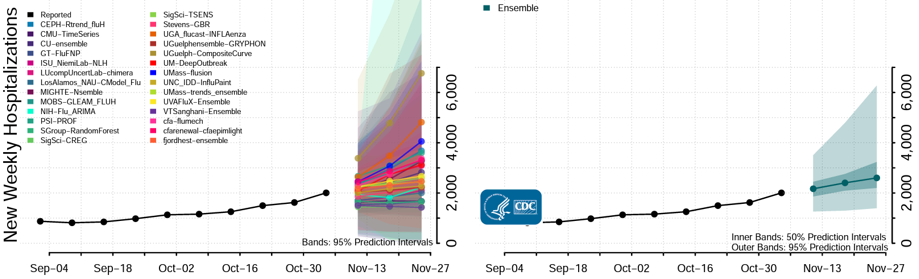
\includegraphics[scale=.55]{Images/national_official_forecasts.PNG}
    \caption{United States flu hospitalization forecasts from multiple 
    competing forecast teams (left) for 1-4 week ahead horizons from the week 
    of November 6, 2023 and an ensemble forecast (right) made by combining all 
    competing forecasts into one. Image downloaded from 
    https://www.cdc.gov/flu/weekly/flusight/flu-forecasts.htm}
    \label{fig:cdc_forecasts}
\end{figure}

There are many methods for constructing an ensemble forecast including but not 
limited to linear and nonlinear methods \cite[]{yao2018using,
geweke2011optimal,hall2007combining,bassetti2018bayesian,
gneiting2013combining,ranjan2010combining} which combine
probability density/mass functions (PDF), cumulative distribution functions 
(CDF), or quantile functions \cite[]{lichtendahl2013better}. The focus in this 
manuscript is on combining forecasts via \textit{linear pooling}, also known as 
model stacking \cite[]{yao2018using,geweke2011optimal,hall2007combining,
stone1961opinion}. Most linear pooling combination methods involve selecting 
a set of combination weights, a point on the simplex, which optimize the 
ensemble according to some criteria but which lack any measure of weight
uncertainty in the optimization. Weights in an ensemble may also be selected 
by maximizing a likelihood or via a Bayesian posterior distribution, but when 
so constructed ensemble forecasts may not be suited for the problem specific 
criteria under which forecasts are assessed. Bayesian model probabilities may 
be used to select weights, but this may also not be well 
suited to problem specific needs. An important case of linear pooling is 
combining via a simple average over the forecasts. This equal weighting (EQW) 
scheme frequently outperforms sophisticated combination methods leading to 
what is known as the 
``forecast combination puzzle'' \cite[]{frazier2023solving,
claeskens2016forecast,smith2009simple}. 


In this manuscript, we introduce a new method which we call the stacked 
Gibbs posterior (SGP), for combining probabilistic forecasts by optimizing a 
linear pool. The SGP provides uncertainty quantification of the weights in 
the ensemble and allows the use of a prior distribution to inform or 
influence the optimized weights. 
The SGP belongs within the \textit{focused Bayesian prediction} (FBP) framework
introduced by Loaiza-Maya et al. \cite[]{loaiza2021focused}. 
In FBP, model parameters and forecasts are attained by constructing a Gibbs 
posterior which is a type of posterior probability distribution constructed 
not within the standard Bayesian framework but by specifying a risk function 
which one desires to optimize in place of a standard likelihood function 
\cite[]{martin2022direct,bissiri2016general}. In a Gibbs posterior, a prior
distribution is assigned to model parameters, and parameter uncertainty is
updated via Bayes theorem. In \cite[]{loaiza2021focused}, the Gibbs posterior
uses a risk function based on proper scoring rules so as to produce optimal
probabilistic 
forecasts. In \cite[]{frazier2025loss} this is extended by fitting
the Gibbs posterior via variational Bayes and showing both theoretically and 
empirically that VB predictions are similar to predictions made via Markov
chain Monte Carlo posterior sampling.

Herein the SGP elaborates upon FBP, but FBP is extended in two important ways.
The risk function optimized in the SGP is based on the continuous ranked 
probability score (CRPS), and it is used to optimize a linear pool of 
an arbitrary finite number of continous forecasts. 
This scenario is considered in section 4.1 of \cite[]{loaiza2021focused}, 
but the number of components in the 
linear pool components is limited to two. In section 5.2 of 
\cite[]{frazier2025loss}, a linear pool of 20 normal component models is
optimized via FBP, but optimization of the CRPS was explicitly excluded 
as a formula for evaluating it was unavailable. Herein we use a closed form
solution of the CRPS over a linear pool of a finite number of normal component
models. We also present a novel definition of the CRPS which allows for
Monte Carlo approximation when the distribution evaluated is a finite mixture
distribution with continuous components. This makes fitting the SGP possible
when distributions of individual forecasts in a linear pool can be sampled from.
The second important extension is the use of a discount factor in the the risk
function. When data to be forecast is dynamic in nature, the discount factor
is used to downweight the influence of data from the distance past and 
upweight more recent data in the forecast optimization. The discount factor
used in the SGP is similar to that used in 
\cite[]{bernaciak2024loss,koop2013large, raftery2010online}.
More details of these two extensions are given in section \ref{sec:sgp}.

The remainder of the manuscript is organized as follows.
Section \ref{sec:preliminaries} includes a brief 
review of probabilistic forecasts and linear pool combinations of forecasts. 
In section \ref{sec:sgp} the SGP is developed, and important details of the 
Gibbs posterior and proper scoring rules are covered. Section 
\ref{sec:simulation} includes three simulation studies to analyze the SGP and 
compare it with other forecast combination methods. In these studies the SGP 
outperforms model averaging and EQW methods for combining forecasts. In section
\ref{sec:flu_analysis} the SGP is used to construct ensemble forecasts for the 
FluSight project where it also outperforms model averaging and EQW approaches. 
The manuscript is concluded in section \ref{sec:4conc}. 



% \section{Situation}

% Consider the case where one is given data $\mathcal{Y} = (Y_1, ..., y_N)$ and a set of $K$ statistical models $\mathcal{M} = (M_1, ..., M_K)$. The intent of each model $M_k$ is to predict a new data point $\tilde{Y}$.
% In most practical situations this is an $\mathcal{M}$-open setting where none of the $K$ models is equal to the true data generating distribution. For each model, it's unknown how $Y_i$ was used to inform the model, and it's possible that additional external data were used. The goal is to create an linear ensemble model of the models in $\mathcal{M}$

% \[
%   p^{(E)}(y) = \sum_{k = 1}^K w_k p_{M_k} (y)
% \]
% by selecting weights $w_k$ which are optimal according to some scoring rule $S(p^{(E)}, y)$. $S(\cdot, \cdot)$ is chosen to be the CRPS. The weights $w_k$ are chosen as from the Gibbs posterior

% \[
% \pi^{(\eta)}(\theta) \propto \text{exp}\{-\eta n R_n(\theta)\} \pi(\theta)
% \]
% where 

% \[
%   R_n(\theta) = \frac{1}{n} CRPS(P^{(E)}, y_n)
% \]
% Here $\theta = \textbf{w} = (w_1, ..., w_k)$. 

\section{Probabilistic forecasts and linear pooling} \label{sec:preliminaries}

We consider the situation where a set of time indexed data $y_1,..., y_T$ 
is given, and one 
is tasked with producing a probabilistic forecast for the unobserved 
$\tilde{y}_{T+h}$ for $h$ time steps ahead of the latest observed time $T$. The 
forecaster produces a forecast $P$ which is probabilistic and which 
may also be indexed by $t \in \{1, ..., T\}$. $P$ may be a PDF, CDF, quantile 
function, set of quantiles or intervals, or any other representation used in 
probabilistic forecasting 
\cite[]{wadsworth2023mixture,gneiting2014probabilistic}. For the 
remainder of this paper, unless otherwise stated, we assume $P$ is the CDF 
forecast of a continuous random variable and $p$ is the corresponding PDF. 
\cite{gneiting2007probabilistic} argue that a probabilistic forecast should 
be evaluated based on sharpness subject to calibration. Sharpness refers to 
how concentrated the forecast uncertainties are, and calibration refers to 
the uniformity of the probability integral transform (PIT). 
Sharpness can be evaluated by the width of predictive intervals but is often 
measured by using proper scoring rules.
The PIT is made by evaluating the probabilistic forecast at the true value 
after it is observed. For the CDF $P$, the PIT of the observed 
$y_{T+h}$, $P(y_{T+h})$ should be roughly uniformly distributed if the 
forecast is well calibrated. The PIT is assessed by making and visualizing 
its histogram \cite[]{gneiting2007probabilistic,hamill2001interpretation}.

When in the situation where there are multiple models used to create 
probabilistic forecasts, we define the set of models as 
$\mathcal{M} = (M_1, ..., M_C)$ where $M_c$ is one model and 
$c \in (1,2,...,C)$. We say $M_{\mathcal{T}}$ is the true model which generates 
$\{y_t\}$. The setting where the true model 
$M_{\mathcal{T}} \notin \mathcal{M}$ is referred to as the $\mathcal{M}-$open 
setting \cite[]{yao2018using,bernardo1994bayesian}. In real world problems, it 
is often the case that forecasts belong to the $\mathcal{M}-$open setting. 
Combining the candidate forecasts in this setting is a 
powerful way to improve forecasts and has been done now for over half a 
century \cite[]{wang2023forecast}. 

\subsection{Linear pooling}
The most common method for combining several probabilistic forecasts is known 
as \textit{linear opinion pooling} which is a linear combination of multiple 
probabilistic forecasts. For $C$ candidate forecasts of the event 
$\tilde{y}_{t+h}$, $h$ time steps into the future, %future from an observed time $t$ 
with CDFs $P_{c}(\tilde{y}_{t + h})$ for $c \in (1,...,C)$, a linear pool 
is defined as the mixture distribution in 
(\ref{eq:linp_forc}). Here, the $w_c$ are linear pool weights. 
To be a proper mixture distribution, the weights must 
be constrained such that they are each nonnegative and together sum to 1, or 
$w_c \geq 0$ and $\sum_{c = 1}^C w_c = 1$.

\begin{equation}
 \label{eq:linp_forc}
 \bar{P}_{\omega}(\tilde{y}_{t + h}) = \sum_{c = 1}^C w_c P_c(\tilde{y}_{t + h})
\end{equation}
Given several individual forecasts, the goal of a forecaster in combining them 
via linear pooling is to select the vector of weights 
$\omega = (w_1, ..., w_C)$ in such a way that the ensemble forecast is 
optimized \cite[]{wang2023forecast,stone1961opinion}. 

If the weights in (\ref{eq:linp_forc}) are optimized according to some score 
function, it is known as an 
\textit{optimal prediction pool} \cite[]{geweke2011optimal,hall2007combining}. 
\cite{yao2018using} introduced a semi-Bayesian approach where a leave-one-out 
(LOO) estimator for combination weights consists of LOO posterior predictive 
distributions of candidate forecast models optimized over a proper scoring 
rule \cite[]{gneiting2007strictly}. It is common to select weights which 
minimize the logarithmic score (LogS) \cite[]{li2023bayesian,yao2018using,
geweke2011optimal,hall2007combining} or weights that minimize the CRPS
\cite[]{berrisch2023crps,li2019combining,
thorey2017online}. Both of these scores are negatively oriented proper 
scoring rules. 
More discussion on proper scoring rules is given in section \ref{sec:sgp}. 
Weight selection methods are often tailored to be problem specific, for 
example they may be formulated to be dynamic \cite[]{li2023bayesian,
billio2013time} or to vary at different points on the PDF 
\cite[]{berrisch2023crps}.


Alternatively, weights in (\ref{eq:linp_forc}) might be selected through model 
averaging which \cite{wang2023forecast} emphasize is distinct from forecast 
combination. Forecast combination is combining forecasts with the aim of 
creating an optimal forecast, whereas model averaging determines model 
probabilities and provides a measure of model uncertainty. The most common 
model averaging approach is called Bayesian model averaging (BMA). In BMA a 
prior probability, $p(\mathcal{M}_c)$, is assigned to each model, and the 
posterior model probability is updated as data is observed according to Bayes 
theorem as

\begin{equation}
    \label{eq:bma}
    p_{BMA}(\mathcal{M}_c |\boldsymbol{y}_t) = 
    \frac{p(\boldsymbol{y}_t |\mathcal{M}_c)p(\mathcal{M}_c)}{\sum_{j = 1}^C 
    p(\boldsymbol{y}_t |\mathcal{M}_j)p(\mathcal{M}_j)}
\end{equation}
where $\boldsymbol{y}_t$ represents all data observed up to time $t$. 
To forecast a future event $\tilde{y}_{t+h}$, one may formulate a predictive 
mixture distribution of 
the form of (\ref{eq:linp_forc}) where the $c^{th}$ forecast model is 
$P_c(y_{t + h}) = P(y_t | \mathcal{M}_c)$ and the weight given to the model 
is $w_c = p_{BMA}(\mathcal{M}_c | \boldsymbol{y}_t)$ 
\cite[]{raftery1996hypothesis}. In the model combination setting, a major 
drawback of BMA is that when the data is large enough, BMA assigns probability 
1 to a single candidate model and probability 0 to all other models. This is 
demonstrated in \cite{yao2018using} and in a simulation study in section 
\ref{sec:simulation} herein. 
Adaptive variable selection (AVS) is an alternative model averaging method 
introduced by \cite{lavine2021adaptive}, and it falls within the Bayesian 
predictive synthesis framework \cite[]{tallman2024bayesian,mcalinn2019dynamic}. 
In AVS, a prior distribution is assigned to each candidate model, and a Gibbs 
posterior model probability is computed for each model. In AVS, 
posterior updating is based on the exponential of some problem specific 
function, $S(\cdot)$,
% $S:\Theta \times \mathcal{Y} \rightarrow \mathbb{R}$ 
rather than on a model likelihood as in BMA. The AVS model probability is then

\begin{equation}
    \label{eq:avs}
    p_{AVS}(\mathcal{M}_c | \boldsymbol{y}_t) 
    \propto \text{exp}\{ -\eta S(\mathcal{M}_c)\} p(\mathcal{M}_c)
\end{equation}
where $\eta$ is a model tuning parameter to be selected based on the needs of 
the problem. AVS allows for much more flexibility in updating posterior model 
averages, but as we show in a simulation study 
in section \ref{sec:simulation} AVS 
may, like BMA, tend to prefer one candidate model over the others.

Among all weight selection methods for linear pooling, one of the most 
consistently well performing combinations is to give equal weight to all 
models in (\ref{eq:linp_forc}) so that $w_1 = w_2 = ... = w_C = 1/C$. This 
phenomenon has received much attention (see for example 
\cite{frazier2023solving,claeskens2016forecast,smith2009simple}), 
and fitting a simple average is obviously easier than using most weight 
optimization methods. Thus for another weight selection method to be worth 
implementing, it should outperform the EQW scheme. It has thus been recommended 
that an EQW average be used as a baseline by which other methods 
are compared 
\cite[]{li2023bayesian,clemen1989combining}.



% \begin{itemize}
%     \item Use equal weights as baseline (Li et al. 2022, Stock \& Watson 2004, Clemen 1989)
%     \item More literature on puzzle in point forecasts (Xiaoqian 2023, Frazier et al. 2024)
%     \item Minimize CRPS (Thorey et al. 2017, Berrisch & Ziel 2021, li 2019, Raftery et al. 2005)
%     \item Time dependent weights (Li et al. 2022)
%     \item Weights specific to problem (Mcalinn West 2019, Lavine 2021, Tallman & West 2024)
%     \item Bayesian (BMA, Lavine 2021, Tallman & West 2024, Yao 2018?not really Bayesian)
% \end{itemize}


\section{Stacked Gibbs posterior} \label{sec:sgp}

For weight selection of a linear pooled ensemble forecast, the stacked Gibbs 
posterior (SGP), introduced in this section, is used to estimate forecast 
combination weights $\boldsymbol{\omega}$, 
the vector of weights in the linear pool of 
(\ref{eq:linp_forc}). The SGP is defined in (\ref{eq:sgp}) and consists of 
three  components, including a prior distribution on $\boldsymbol{\omega}$, 
$\pi(\boldsymbol{\omega})$, 
an empirical risk function $S_n(\cdot)$ based on a proper scoring rule, and a 
tuning parameter $\eta$. Each of these is discussed in further detail in 
sections \ref{sec:gibb_post} and \ref{sec:prop_score}.

\begin{equation}
    \label{eq:sgp}
    \pi^{(\eta)}_n (\boldsymbol{\omega}) \propto 
    \text{exp}\{-\eta n S_n(\boldsymbol{\omega})\} 
    \pi(\boldsymbol{\omega})
\end{equation}

The SGP is a probability distribution over the simplex
which allows for inferential 
analysis of the weights. This is in contrast to the stacking done by 
\cite{yao2018using} where the weights are optimized as a point on the simplex. 
The SGP also differs from the posterior model averaging in (\ref{eq:bma}) and 
(\ref{eq:avs}) where the posterior 
probability is point assigned directly to the loss functions of 
individual candidate models rather than 
to the model weights of the linear pool as a whole. 
The SGP is a specific case of FBP where the risk function is the CRPS evaluated
over a linear pool of an arbitrary number of continous model components. 
As far as we are aware, methods for evaluating the risk function have been 
available only in the case of a two component linear pool model. In this 
section, we provide a new definition of the CRPS which allows for evaluation
of the CRPS for a linear pool of any finite number of continuous 
model components.
In the remainder of this section a general Gibbs posterior is defined in 
more detail following \cite{martin2022direct}, discussion of the use of a
discount factor is given, proper scoring rules are 
defined following \cite{gneiting2007strictly} with specific emphasis on the 
CRPS, and a posterior consistency result is presented. 

\subsection{Gibbs posterior} \label{sec:gibb_post}

The standard Bayesian posterior distribution for an unknown parameter 
$\theta$ given some data $y$ is defined by Bayes theorem as 
$\pi(\theta | y ) = c L(y|\theta) \pi(\theta)$
so that $\pi(\theta|y)$ is equal to the joint distribution of a statistical 
model $L(y|\theta)$ and a prior distribution $\pi(\theta)$ times a normalizing 
constant $c$. When the model $L(y|\theta)$ does not exist or the goal is 
inference on parameters which minimize some loss function rather than 
maximize a likelihood, the Gibbs posterior is a alternative to the standard 
posterior distribution which allows for inference on the minimizer of a 
selected function. The Gibbs posterior has been used in many applications, 
and has shown promising results, often outperforming the Bayesian posterior 
in question specific parameter estimation, prediction, model selection, and 
model averaging \cite[]{martin2022direct,loaiza2021focused,
lavine2021adaptive,syring2017gibbs,jiang2008gibbs}.


Following \cite{martin2022direct}, the setup for constructing a Gibbs posterior 
is as follows. We are given data, 
$y_1, ..., y_n \in \mathcal{Y}$ typically assumed to be independent and 
identically distributed (i.i.d.) from some inaccessible distribution 
$\mathcal{L}$. We do not assume a likelihood model for the data, either 
because one is not available or because inference via a likelihood is not 
useful for the problem. Instead we define a loss function parameterized by 
$\theta \in \Theta$, 
$l_{\theta}(y) : \Theta \times \mathcal{Y} \rightarrow \mathbb{R}$. 
Two common loss functions are the squared-error and the absolute-error losses. 
The goal for prediction is to minimize the loss function. 


A risk function $R(\theta)$ is the expectation of the loss function 
$l_{\theta}(y)$ over the distribution $\mathcal{L}$, or 
$R(\theta) = E l_{\theta}(Y)$, where $E$ denotes the expected value with 
respect to the true data generating distribution of $y_i$.
Primarily, interest is in the risk minimizer 
$\theta^*$ defined in (\ref{eq:risk_min}) where $\in$ indicates that 
$\theta^*$ may not be unique.

\begin{equation}
    \label{eq:risk_min}
    \theta^* \in \underset{\theta \in \Theta}{\mathrm{argmin}} R(\theta)
\end{equation}
Since $R(\theta)$ is inaccessible, an empirical risk function $R_n(\theta)$ 
based on the given data is formulated in (\ref{eq:emp_risk}). Then 
$\hat{\theta}_n$, an estimate of $\theta^*$,  is estimated by the estimator 
in (\ref{eq:emp_risk_min}).  

\begin{equation}
\label{eq:emp_risk}
    R_n(\theta) = \frac{1}{n}\sum_{i = 1}^n l_{\theta}(y_i)
\end{equation}

\begin{equation}
    \label{eq:emp_risk_min}
    \hat{\theta}_n \in \underset{\theta \in \Theta}{\mathrm{arg min}} R_n(\theta)
\end{equation}
The estimator can be viewed as an $M$-estimator, the statistical properties 
of which have been extensively studied \cite[]{boos2013essential, 
van1998asymptotic}. 







The purpose of the Gibbs posterior is to produce probabilistic uncertainty 
for the unknown risk minimizer. In this setting, the Gibbs 
posterior is defined in (\ref{eq:gibb_post}) where $R_n(\theta)$ 
is the empirical 
risk from (\ref{eq:emp_risk}). The Gibbs posterior is proportional to the 
product of a prior distribution assigned to $\theta$ and the exponential of 
the empirical risk times a parameter $\eta > 0$ which \cite{martin2022direct} 
refer to as the \textit{learning rate}. 

\begin{equation}
    \label{eq:gibb_post}
    \pi^{(\eta)}_n (\theta) \propto \text{exp}\{-\eta n R_n(\theta)\} 
    \pi(\theta)
\end{equation}


The learning rate $\eta$ is a tuning parameter used to control the balance 
between the prior distribution and the data. It should not be considered a 
model parameter to which one may assign a prior, but rather should be 
selected by a data driven tuning or some other problem specific selection. 
Often the learning rate is tuned so that posterior credible intervals have 
frequentist coverage probability, or it is selected via cross validation to 
optimize some criteria \cite[]{martin2022direct,syring2017gibbs,
bissiri2016general,zhang2006information}. 
While the tuning of $\eta$ may have a noticeable effect on predictive
performance for small sample sizes,
it was recently argued in \cite[]{mclatchie2025predictive} that for moderate
to large sample sizes, the selection of $\eta$ will have little effect on 
predictive accuracy.
Importantly the asymptotic 
consistency of the Gibbs posterior is not dependent on $\eta$, so selecting 
$\eta$ by most well reasoned methods should be appropriate 
\cite[]{martin2022direct,loaiza2021focused}.







For the SGP in (\ref{eq:sgp}), the more general $\theta 
\in \Theta$ is replaced with $\omega \in \{w_1, ..., w_C : 0 \leq w_c \leq 1, 
\sum_c w_c = 1\}$, and we consider empirical risk functions based on one of 
two loss 
functions. The first of these functions is in (\ref{eq:er_iid}), and is used 
for the simple case of i.i.d. data $y_1,..., y_n$ and candidate models which 
are provided once and remain constant as more data become available.

\begin{equation}
    S_n(\omega) = G_n(\omega) = \frac{1}{n}\sum_{i = 1}^n 
    G(\bar{P}_{\omega}, y_i).
    \label{eq:er_iid}
\end{equation}
Here $\bar{P}_{\omega}$ is the CDF of an ensemble forecast with $C$ 
competing forecast models from (\ref{eq:linp_forc}). Each component $P_c$ 
is fully specified, so that the only parameters to be estimated are model 
weights. The function $G(\cdot, \cdot)$ is a proper scoring rule 
(see section \ref{sec:prop_score}).
A second empirical risk, used in a time dynamic setting is given in 
(\ref{eq:er_dyn}). Here we have an observed time series $y_1, ..., y_T$, and 
we want to construct an ensemble model for forecasting the future observation 
$\tilde{y}_{T+h}$. 

\begin{equation}
   S_T(\omega) = G_T(\omega) = \frac{1}{T}\sum_{t = 1}^T \alpha^{T-t} 
   G(\bar{P}_{t, \omega}, y_t)
    \label{eq:er_dyn}
\end{equation}
In this dynamic setting, $0 < \alpha \leq 1$ is a discount factor 
used to lessen the influence of 
previous forecasts making the performance of the most recent forecasts 
the most influential. For example, if $\alpha = 0.98$, 
observations from 10 time steps in the passed
receive approximately 83\% of the weight as the most recent value.
If $\alpha = 1$, the risk function in 
(\ref{eq:er_iid}) is recovered.

Discount factors (also known as forgetting factors)
have been used in the model averaging setting but not
to our knowledge in the FBP setting 
\cite[]{bernaciak2024loss,lavine2021adaptive, zhao2016dynamic, 
koop2013large,raftery2010online}. 
The discount
factor has been largely used to improve upon BMA which is best for static 
data as opposed to dynamic data. Previous literature suggests $\alpha$ 
between 0.95 and 0.99 leads to more accurate predictions, and that varying 
$\alpha$ has little effect except where there are dramatic changes in the 
time series \cite[]{lavine2021adaptive, koop2013large}. 
In the dynamic analyses below
below we also tried other values of $\alpha$ between 0.9 and 0.99 but 
found the specific value made little difference in predictive performance.
In \cite{lavine2021adaptive}, the discount factor is 
fixed at $\alpha = 0.98$, and we use the same value herein. 

The linear pool 
$\bar{P}_{t, \omega}$ is made up of competing models which may or may not be 
time dependent. In the second simulation in section \ref{sec:simulation}, 
the risk in (\ref{eq:er_dyn}) is used where competing models are fixed in 
time whereas in both the third simulation study and 
the analysis of flu forecasts in section 
\ref{sec:flu_analysis}, the forecasts vary in time.





\subsection{Proper scoring rules and the continuous ranked probability score} 
\label{sec:prop_score}

In this subsection, we review the definition of a proper scoring rule and 
give the definitions for the LogS and the CRPS. Also included are additional 
properties of the CRPS. 
Following \cite{gneiting2007strictly}, a scoring rule is a function 
$G:\mathcal{P} \times \mathcal{Y} \rightarrow [-\infty, \infty]$ where 
$\mathcal{P}$ is a convex class of probability measures on 
$(\mathcal{Y}, \mathcal{A})$, $\mathcal{A}$ being a $\sigma$-algebra on the 
set $\mathcal{Y}$.  $G(P, y)$ is then a score on how well a predictive 
distribution, typically a probabilistic forecast, $P \in \mathcal{P}$ 
predicts a realized value $y$ on the sample space. A negatively oriented 
scoring rule is a proper scoring rule if for two forecasts 
$P, Q \in \mathcal{P}$, the function $G(P, Q) = \int G(P, y)dQ(y)$ is such 
that $G(Q,Q) \leq G(P,Q)$. If the inequality is strict, then $G(\cdot, \cdot)$ 
is a \textit{strictly proper scoring rule}.

 Proper scoring rules are used not only to score probabilistic forecasts but 
 as functions to optimize over when selecting weights for an optimal linear 
 pool \cite[]{lavine2021adaptive,li2019combining,yao2018using,
 thorey2017online,geweke2011optimal}. 
In practice, a number of scoring rules for continuous distributions are used 
to estimate parameters and evaluate forecasts 
\cite[for some examples]{gneiting2014probabilistic, gneiting2007probabilistic}, 
the LogS being perhaps the most widely used. The LogS is defined in 
(\ref{eq:logs}) and evaluates a distribution by its PDF $p$. 

\begin{equation}
    \label{eq:logs}
    \text{LogS}(p, y) = -\text{log}(p(y))
\end{equation}
The CRPS is an increasingly popular scoring rule which, depending on the 
application, has certain advantages over the LogS. The CRPS is a global 
scoring rule in that it evaluates the whole distribution of a forecast 
whereas the LogS is a local scoring rule in that it evaluates the distribution 
only at a point \cite[]{gneiting2014probabilistic}. When used for estimation, 
the CRPS is often a more robust estimator than the LogS and can lead to 
sharper and better calibrated forecasts under model misspecification 
\cite[]{gebetsberger2018estimation,gneiting2005calibrated}. The CRPS is 
defined in (\ref{eq:crps}) and evaluates a distribution through its CDF $P$.


\begin{equation}
    \label{eq:crps}
    \text{CRPS}(P, y) = \int_{-\infty}^{\infty} (P(x) - \mathds{1}
    (y \leq x))^2 dx
\end{equation}
For $P$ belonging to certain distribution families, there may be a closed 
form solution to (\ref{eq:crps}) (see table 1 of \cite{zamo2018estimation}). 
Particularly relevant for the work herein is the closed form solution of the 
CRPS when $P$ is a mixture distribution with normal components. 
\cite{li2019combining} provide the derivation for the normal mixture CRPS 
in (\ref{eq:norm_mix_crps}).

\begin{equation}
\begin{aligned}
    \label{eq:norm_mix_crps}
     CRPS(P, y) &= \sum_{c = 1}^C \sum_{c' = 1}^C \alpha_{c, c'}w_c w_{c'} + 
     \sum_{c = 1}^C \beta_c w_c; \quad \text{ where}\\~  \\
        \alpha_{c,c'} = &-\frac{1}{\sqrt{2\pi}}\sqrt{\sigma_c^2 + 
        \sigma_{c'}^2} \text{exp} 
        \left( \frac{(\mu_c - \mu_{c'})^2}{2 (\sigma_c^2 + 
        \sigma_{c'}^2)}\right) \\
        &-\frac{\mu_c - \mu_{c'}}{2}\left[2 \Phi 
        \left(\frac{(\mu_c - \mu_{c'})}{\sqrt{\sigma_c^2 + 
        \sigma_{c'}^2}}\right) - 1 \right] \\
        \beta_c = &\sqrt{\frac{2}{\pi}}\sigma_c 
        \text{exp}\left(-\frac{(\mu_c - y)^2)}{2\sigma_c^2}\right) \\
        &+ (\mu_c - y) \left[2\Phi\left(\frac{\mu_c - y}{\sigma_c}) 
        \right) - 1\right] 
\end{aligned}
\end{equation}

The CRPS has some general forms other than (\ref{eq:crps}) including 
(\ref{eq:crps_mse}) which was shown by \cite{gneiting2007strictly}.

\begin{equation}
    \label{eq:crps_mse}
    \text{CRPS}(P, y) = E|X -y| - \frac{1}{2} E|X - X'|
\end{equation}
Here $X$ and $X'$ are independent copies of the same random variable with 
CDF $P$. When there is no closed form solution to the CRPS but where one 
can sample from the forecast distribution, the CRPS may still be estimated 
via Monte Carlo approximation by estimating the expectations in 
(\ref{eq:crps_mse}). For the cases where $P$ takes the form of an ensemble 
forecast where all components are continuous distributions, we contribute the
additional reduction of
(\ref{eq:crps_mse}) to (\ref{eq:crps_ens_mse}) found in proposition 
\ref{prop:crps_ens_mse}. A 
proof for proposition \ref{prop:crps_ens_mse} 
is in appendix \ref{app:crps_ens_pf}. 

\begin{proposition}
Given $C$ CDFs of continuous distributions $P_1, ..., P_C$ and 
a set of weights on a simplex $w_1, ..., w_C$, the CRPS of the mixture
distribution with CDF $\bar{P}(x) = \sum_c w_c P_c (x)$ evaluated at $y$ has
the form of equation (\ref{eq:crps_ens_mse}).
\begin{equation}
    \label{eq:crps_ens_mse}
    CRPS(\bar{P}, y) = \sum_{c = 1}^C w_c E|X_c - y| - 
    \frac{1}{2}\sum_{c = 1}^C \sum_{c' = 1}^C w_c w_{c'} E|X_c - X_{c'}|
\end{equation}
Here $X_c$ is a random variable with corresponding CDF $P_c$, and $X_{c'}$ is 
a random variable independent of $X_c$ but which is equal in distribution.
\label{prop:crps_ens_mse}
\end{proposition}
\cite{li2019combining} showed this result for all mixture components being 
Gaussian, but it's simple to show that it holds when all components are 
continuous. This result allows for straightforward CRPS estimation for a 
continuous mixture distribution forecast when samples of the component 
distributions are available. 
% It's also useful for showing the CRPS is a convex function, an important point for proving theorem \ref{thm:sgp_cons} below (see appendix \ref{app:sgp_cons_pf}).
To complete the definition of the SGP in (\ref{eq:sgp}), we let the function 
$G(\cdot, \cdot) = CRPS(\cdot, \cdot)$ and $G_n$ take the form of either 
(\ref{eq:er_iid}) or (\ref{eq:er_dyn}).

\subsection{SGP consistency}
When using the SGP to produce forecasts, one would like assurance
that the optimized weights converge to create a linear pool which produce the
best forecasts subject to the CRPS. The consistency result in this section
provides some of that assurance. We note that similar results under
differing conditions were shown 
in \cite[]{frazier2025loss} and 
in \cite[]{loaiza2021focused}.

In \cite{martin2022direct}, parameter asymptotic consistency results of the 
Gibbs posterior similar to consistency results pertaining to the standard 
Bayesian posterior are established, and minimal conditions for consistency 
are given for i.i.d. data. The difference for the Gibbs posterior is that 
the posterior mass converges to the risk minimizer. The conditions for 
consistency follow the conditions for consistency in $M$-estimation 
\cite[]{van1998asymptotic}. We define posterior consistency in 
\ref{def:cons} which is the same definition used by \cite{martin2022direct}.

\begin{definition}
\label{def:cons}
For a given distance $d:\Theta \times \Theta \rightarrow \mathbb{R}^+$, 
the Gibbs posterior distribution $\pi_n^{(\eta)}$ is consistent at 
$\theta^*$ if
\[
    \pi_n^{(\eta)}(\{\theta : d(\theta, \theta^*) > \epsilon\}) \rightarrow 0
    % \text{ in probability, as } n \rightarrow \infty
\]
in probability as $n \rightarrow \infty$
\end{definition}

% \begin{definition}
%   yourmom.
% \end{definition}

For the SGP in (\ref{eq:sgp}) with the empirical risk function in 
(\ref{eq:er_iid}) the posterior consistency is shown for the distance 
function being the Euclidean distance, 
$d(\boldsymbol{a}, \boldsymbol{b}) = ||\boldsymbol{a} - \boldsymbol{b}||$, 
and the prior distribution on the weight vector $\boldsymbol{\omega}$ 
to be the Dirichlet 
distribution $\pi(\boldsymbol{\omega}) \sim Dirichlet(\lambda)$. 
Other distance functions 
and prior distributions may work, but importantly one of the conditions for 
consistency is that the prior distribution gives sufficient mass to the risk 
minimizer or that $\pi(\{\theta:R(\theta) - R(\theta^*) < \delta \}) > 0$ 
for all $\delta > 0$. The support of the Dirichlet distribution is over the 
simplex and thus meets this condition. For i.i.d. data $y_1, ..., y_n$ with 
probability law $\mathcal{L}$ where $E|Y| < \infty$ and where the empirical 
risk function is the function in (\ref{eq:er_iid}), posterior consistency of 
the SGP proposed in (\ref{eq:sgp}) is affirmed by theorem \ref{thm:sgp_cons}. 

\setcounter{theorem}{0}
% \stepcounter{theorem}


\begin{theorem}
\label{thm:sgp_cons}
     
     If $\boldsymbol{\omega}^* \in \Omega = \{w_1, ..., w_C : 
     \sum_c w_c = 1, 0 \leq w_c \}$ uniquely minimizes $G(\omega) = 
     E[CRPS(\bar{P}_{\omega}, Y)]$ and for the prior distribution $\pi$, 
     $\pi(\{\boldsymbol{\omega} : G(\boldsymbol{\omega}) - 
     G(\boldsymbol{\omega}^*) < \delta\}) > 0$ 
     for all $\delta > 0$, then for any $\epsilon > 0$

     \[
        \pi_n^{(\eta)} (\{\boldsymbol{\omega} : 
        d(\boldsymbol{\omega}, \boldsymbol{\omega}^*) > \epsilon \} ) 
        \rightarrow 0
     \]
     in $\mathcal{L}$-probability as $n \rightarrow \infty$
\end{theorem}



Theorem \ref{thm:sgp_cons} shows that as more data is observed, 
the SGP becomes more
concentrated around the unique minimizer $\boldsymbol{\omega}^*$. Thus, at 
least in the case of i.i.d. data, the SGP will converge to produce the best
possible linear pool combination for predictive accuracy under the CRPS. 
In theory, this result may also be used to show that the SGP produces better 
predictive results than the standard likelihood Bayesian results.
This manuscript does not include consistency results beyond the case of data 
being i.i.d. and having competing models which are fixed, or unaltered by 
additional data. Such is the setting of the first simulation study in the 
next section. One reason it may be difficult to develop theory in a dynamic 
setting is that the models which have the best predictive abilities may be 
changing in time making $\boldsymbol{\omega^*}$ a 
moving target. However, this does not 
necessarily discount the SGP's ability to select model weights which produce 
well performing ensemble forecasts in dynamic settings. This is explored in 
additional simulation studies and in a real data example below.







\section{Simulation studies} \label{sec:simulation}

This section contains three simulation studies to demonstrate the SGP's ability 
to estimate optimal weights for model combination. The first study is done in 
an i.i.d. data setting with fixed competing predictive models. The second study 
includes the same predictive models, but the data is generated dynamically and 
weights are optimized for one step ahead forecasts. The third study focuses on
combining four models used to forecast data generated from the stochastic
compartmental susceptible-infectious-recovered (SIR) disease outbreak model.
Unless stated otherwise, the prior distribution used for the SGP was an
uninformative Dirichlet distribution with the parameter being a vector of 1s.
In all studies, the weights used in the SGP ensembles are selected as the 
mean vectors of 
individual draws from the Gibbs posterior obtained  Hamiltonian 
Monte Carlo sampling using the \texttt{cmdstanr} \texttt{R} package 
\cite[]{stan2024manual,gabry2022stan}.


\subsection{I.I.D. data}

This first shows how the SGP may be used to optimize 
weights among competing models in an $\mathcal{M}$-open scenario and is similar 
to the first simulation study in \cite{yao2018using}. In this study there are 
six candidate models for predicting the data. Data is generated from the 
mixture of normals distribution 
$\nu \times N(3, 1) + (1 - \nu) \times N(6.5, 1)$ where $\nu = 0.65$. 
Because all simulated data is i.i.d., the empirical risk function from 
(\ref{eq:risk_min}) is used, and the consistency results from theorem 
\ref{thm:sgp_cons} hold. The six competing models are each normally 
distributed with variance 1, but each model has a unique mean parameter, 
the unique means being $\{0, 2, 4, 6, 8, 10\}$. Figure \ref{fig:iid_sym_examp}
% \spencer{(may put in supplementary materials)}
shows in black the mixture distribution from which data is simulated as well as 
the candidate normal predictive models in grey. 


\begin{figure}[hbt!]
    \centering
    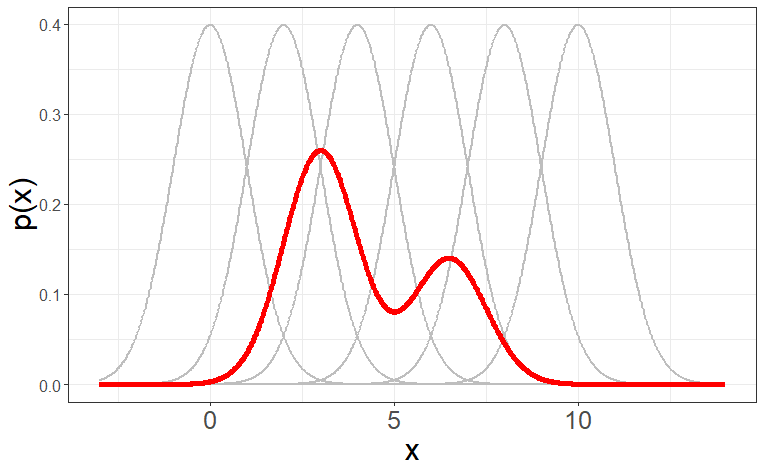
\includegraphics[scale = .17]{Images/iid_sym_examp.png}
    \caption{Mixture distribution density function from which data are 
    simulated (black) and 6 candidate normal predictive densities (grey). 
    The mixture distribution is 
    $\nu \times N(3, 1) + (1 - \nu)\times N(6.5,1); \nu = 0.65$. The candidate 
    predictive distributions are each normal with variance 1 and 
    means 0, 2, 4, 6, 8, and 10.}
    \label{fig:iid_sym_examp}
\end{figure}

The predictive performance of the SGP ensemble 
is compared with that of BMA, AVS, and EQW. For 
both AVS and SGP, the learning rate $\eta$ needed to be selected, and we opted 
to select $\eta$ with the aim of minimizing the CRPS for prediction. A figure
in the supplementary materials shows an example of how the 
CRPS varies for different 
values of $\eta$ for the AVS and SGP \cite{wadsworth2025bayesstack}. In the 
case of AVS, LOO cross 
validation over a grid of values for $\eta$ was performed and the $\eta$ 
which minimized the predictive CRPS was selected. Additional details on the 
cross validation performed here are available in the supplementary materials.
For the SGP, the value of 
the CRPS continues to decrease as $\eta$ increases. The improvement became 
less stark for higher values, so $\eta$ was fixed at 15 so as to retain 
influence from the prior distribution.



Figure \ref{fig:opt_dens} %(\spencer{put in supplement?})
shows examples from estimating model weights of 
constructing a linear pool from the candidate models for samples sizes of 10, 
20, 50, 100, and 200 for BMA, AVS, EQW, and SGP weight selection methods. 
The top 
row shows how with a sample size as small as 10, BMA concentrates nearly all 
model probability into one model. AVS does better at spreading the model 
probability around, but as the sample size increases, it too will often favor 
one model over all others. SGP on the other hand tends to better capture the 
spread of the true distribution as the sample size increases.


\begin{figure}[hbt!]
    \centering
    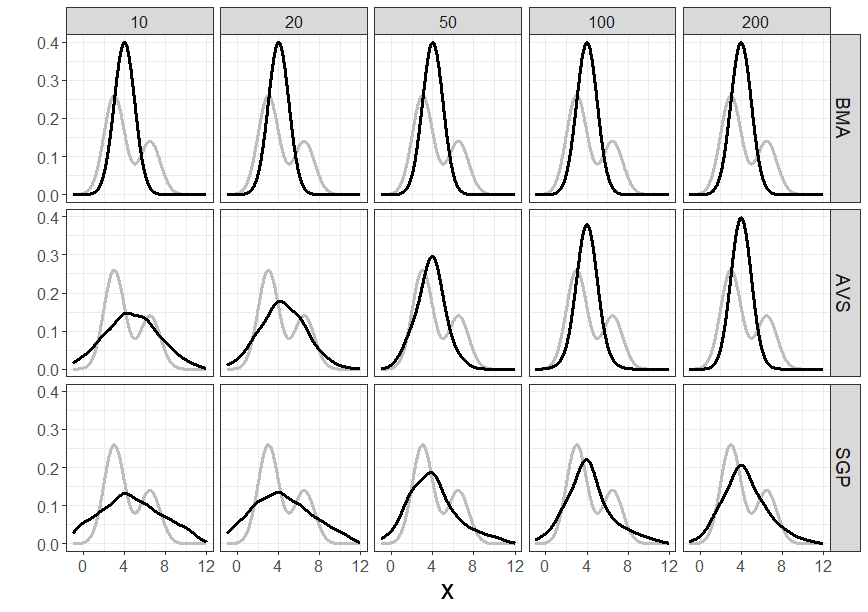
\includegraphics[scale=.2]{Images/iid_sym_density.png}
    \caption{Examples of estimated densities after weighting of competing 
    models faceted by weighting method and sample size. 
    The weighting methods shown include BMA, AVS, EQW, and SGP. The estimated 
    densities (black) overlay the true model density (grey).}
    \label{fig:opt_dens}
\end{figure}


Figure \ref{fig:iid_scores} shows boxplots of the CRPS and the LogS for the 
four competing weight selection methods. 
The simulation was replicated 500 times for 
each sample size, and after selecting weights, the CRPS and LogS in these plots 
were calculated as the Monte Carlo mean scores for 1,000 additional draws from 
the true distribution after selecting weights. As the sample size increases, 
the SGP clearly separates itself from the model averaging approaches. AVS 
appears to perform well for smaller sample sizes but worsens as the sample 
size increases, and it tends to favor one model over the others. 


\begin{figure}[hbt!]
\centering
  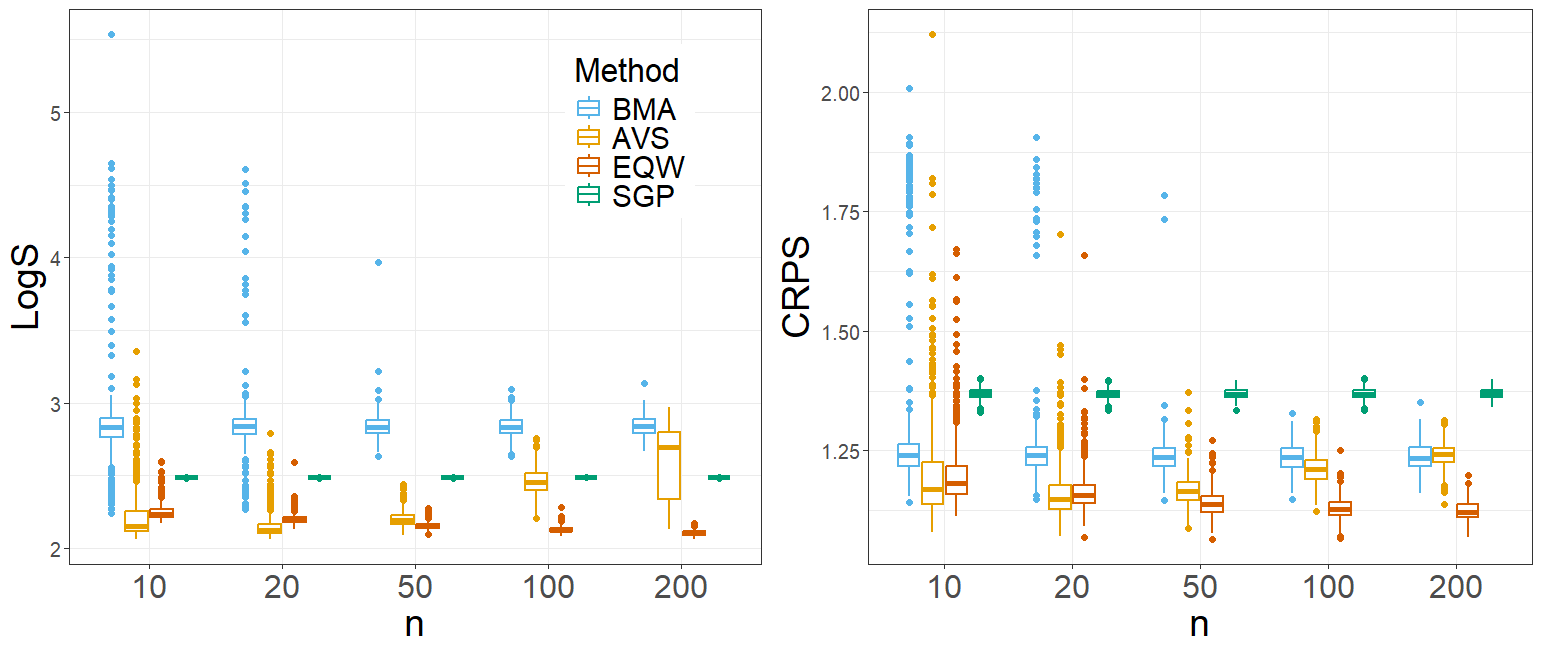
\includegraphics[width=1.1\linewidth]{Images/iid_sim_res_col.png}
\caption{Boxplots of the mean of 1,000 Monte Carlo LogSs (left) and CRPSs 
(right) for 500 replicates and for increasing sample size $n$. 
Plots are colored by weighting method. For both
LogS and CRPS, lower is better. }
\label{fig:iid_scores}
\end{figure}

% \jarad{Include "lower is better".}
% \jarad{Write out CRPS and LogS}
% \jarad{Make n explicit}

\subsection{Dynamic data simulation forecast}

The simulation study in this section has similarities to the previous study 
including that it utilizes the same fixed candidate predictive models and the 
data is simulated from a normal mixture distribution. Here, however, the 
mixture distribution from which the data are simulated is dynamic over time 
and the focus of making an ensemble model is to perform one step ahead 
forecasting. 
The data were simulated from the model in (\ref{eq:dyn_sim_mod}). The two 
component normals in the mixture distribution are the same as in the previous 
study, but here the weights for each model are updated at each time point 
according to a random walk process. 
\begin{equation}
    \begin{aligned}
    \label{eq:dyn_sim_mod}
        Y_t &\sim \omega_{1,t} \times N(3, 1) + \omega_{2,t} 
        \times N(6.5, 1) \\
        \omega_{i,t} &= \frac{\text{exp}(z_{i,t})}{\sum_a \text{exp}(z_{i,t})}; 
        \quad i \in \{1,2\}\\
        \boldsymbol{z}_t &\sim N(\boldsymbol{z}_{t-1}, \sigma^2 I) \\
        (\omega_{1,1}, \omega_{2,1}) &= (0.65, 0.35) \\
        \sigma^2 &= 0.01
    \end{aligned}
\end{equation}
A single observation $y_t$ is simulated at each time step 
$t \in \{1, ..., T = 50\}$, and at each step the ensemble weights are 
selected and an ensemble for forecasting $\tilde{y}_{t+1}$ is constructed. 
A figure 
% \ref{fig:dyn_wts_ex} 
in the supplementary materials
gives an example of the dynamic weights simulated 
from (\ref{eq:dyn_sim_mod}). The left plot shows the simulated weight values, 
and the right plot shows the SGP optimized weights of the competing forecasts 
for times 2 to 50. The empirical risk used for fitting the SGP is that in 
(\ref{eq:er_dyn}). The same discount factor of $\alpha^{T-t}$
is similarly applied to the AVS and BMA methods as done in 
\cite{lavine2021adaptive}.



The performance of the ensemble forecasts is assessed in terms of proper 
scoring rules as well as by the PIT, that is the uniformity of the histogram 
of observations evaluated by the probabilistic forecast. The PIT is evaluated 
both by looking at the PIT histogram and by measuring the distance between the 
PIT and the uniform distribution using the unit Wasserstein distance metric 
(UWD1) from section 3.4 in \cite{wadsworth2025quantile}.
The plots on the left of figure \ref{fig:dyn_sim} show how the CRPS and LogS 
forecasts behave over time for one step ahead forecasts. 
The lines represent the mean scores over the 500 
simulation replicates. Here the SGP outperforms AVS, BMA, and EQW ensembles 
with the superior performance appearing more starkly for LogS than for CRPS. 
Unsurprisingly the EQW forecast scores remain relatively constant through time 
while the other methods improve as time goes on. Interestingly, the behavior 
of AVS shown in the i.i.d. case in the previous study to perform very well 
with small amounts of data but to worsen with larger data does not manifest 
in this study of dynamic forecasting.
The right two plots in figure \ref{fig:dyn_sim} show 
the PIT results for one step ahead forecasts for forecasts of times 2 to 50 
over the same 500 replications of simulated data. The histogram plots clearly 
show that the
SGP PIT histogram is much nearer to uniformity than the PIT histograms for the 
other methods. The boxplots of the 500 UWD1 distances show smaller UWD1 values 
for the SGP PIT meaning the distances between the PIT and the standard uniform 
distribution tend to be smaller for SGP, further showing superior calibration 
compared to the other methods.


% \begin{figure}[hbt!]
% \centering
% %\begin{subfigure}{}
%   % \centering
%   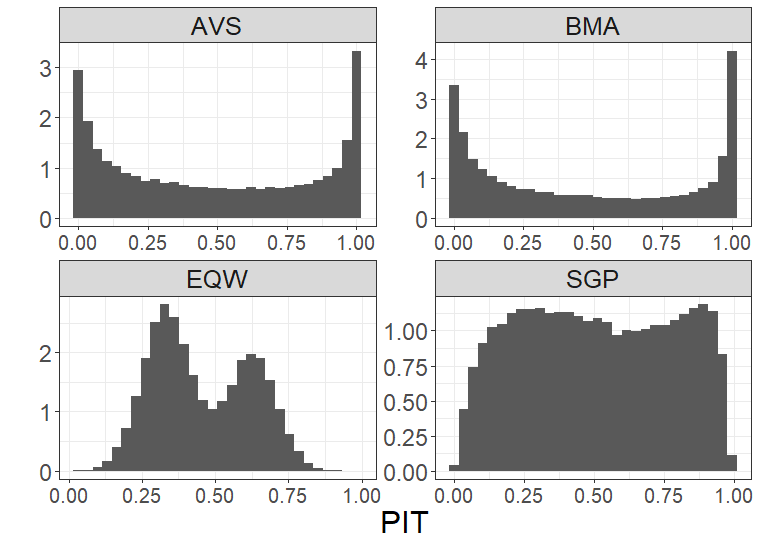
\includegraphics[width=.48\linewidth]{Images/dyn_sim_pit.png}
%   % \caption{A subfigure}
%   % \label{fig:sub1}
% %\end{subfigure}%
% \hspace{0.01\textwidth}
% %\begin{subfigure}{}
%   \centering
%   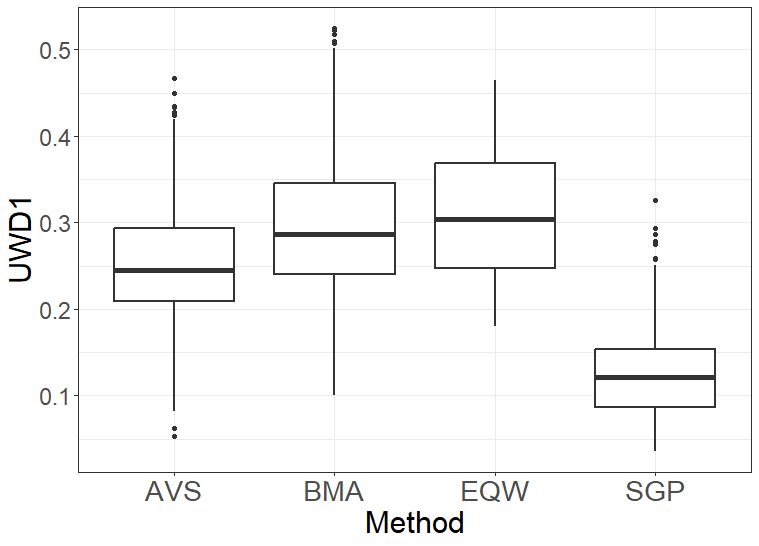
\includegraphics[width=.48\linewidth]{Images/uwd1_box.png}
%   % \caption{A subfigure}
%   % \label{fig:sub2}
% %\end{subfigure}
% \caption{Plots for assessing calibration of one step ahead forecasts for the four weighting methods. The figure shows the PIT for all $99 \times 500$ simulated one-step-ahead forecasts for AVS, BMA, EQW, and SGP (left) and boxplots of the UWD1 distance between a standard uniform distribution and the empirical distribution of the PIT for the weighting schemes for 99 predictions (right).}
% \label{fig:dyn_pit}
% \end{figure}

\begin{figure}[hbt!]
\centering
  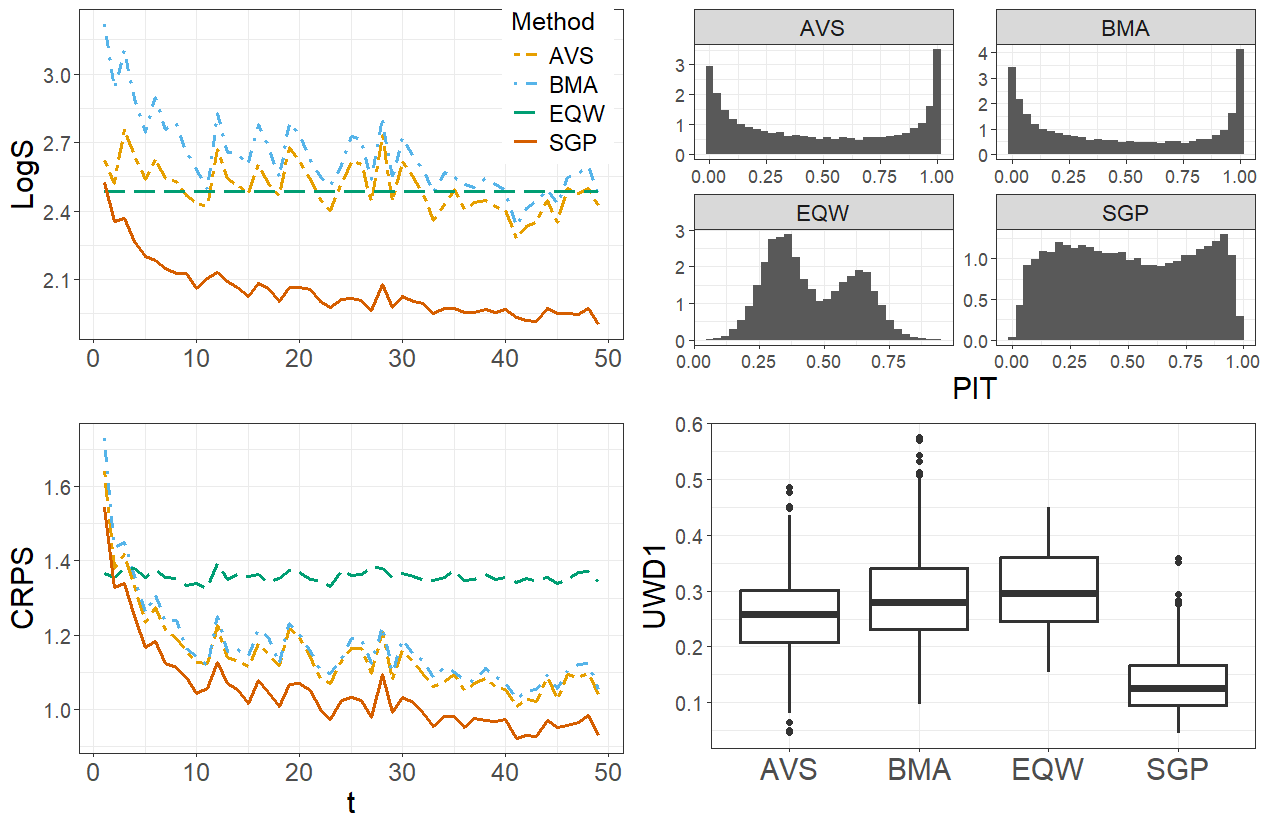
\includegraphics[width=.9\linewidth]{Images/dyn_sim_res_col.png}
\caption{Plots showing results for one step ahead forecasts for dynamically
weighted data for the four
weighting methods SGP, AVS, BMA, and EQW. Two plots show performance
according to proper scoring rules
(left). The mean LogS (top) and CRPS (bottom) over 500 replicates of one step
ahead predictions at 49 time points colored by weighting methods.
The other two plots show calibration according to the PIT (right). The PIT
histogram for all forecasts faceted by weighting method is shown (top), and
boxplots by weighting method of the UWD1 for all forecasts of one simulation
replicate is shown (bottom).}
\label{fig:dyn_sim}
\end{figure}



\subsection{SIR data simulation forecasts}

The SIR compartmental model was introduced by \cite{kermack1927contribution} 
and is a standard mathematical model used for modeling
disease outbreaks. The SIR model models a population in which at any given 
time each individual belongs to one of
three compartments: susceptible, infected, or recovered. The most basic SIR
model is deterministic and defined by a set of ordinary differential equations
--one for each compartment-- but stochastic extensions allow one to simulate
from an SIR model with uncertainty 
\cite[]{allen2008mathematical,widgren2019siminf}. When fitting an SIR model
to track an epidemic, it is common practice to treat real outbreak measurements
as analogous to the values in the infected compartment
\cite[]{widgren2019siminf, osthus2019dynamic}. 
% \spencer{Should I add more details
% about the SIR model, maybe in the supplementary material?}

The data used in this simulation study were generated from a stochastic SIR 
model using the \texttt{SimInf} package in \texttt{R} 
\cite[]{widgren2019siminf}. For each of 3,000 simulation replicates, 35 
consecutive ``weeks`` of infection counts were sampled. Starting at week 5, 
we fit four individual forecast models and used each to make one week ahead 
forecasts of 
infections for each of weeks 6 to 35.
Using the individual forecasts, we used the SGP to construct an 
ensemble forecast and compared the performance to the performances of 
ensembles constructed via the AVS, BMA, and EQW methods. The decision to use
four component forecasts was based on the recommendation from 
\cite{fox2024optimizing} to forecast diseases such as influenza and COVID-19
with an ensemble of four or more components. The four models included 
a Bayesian SIR model similar to that used to forecast the flu in 
\cite{osthus2019dynamic}, a nonlinear Bayesian model similar to that used by 
\cite{ulloa2019} and \cite{wadsworth2025forecasting}, an ARIMA model fit 
using the \texttt{forecast} package in \texttt{R} 
\cite[]{hyndman2008automatic}, and a naive random walk model also fit using
the \texttt{forecast} package. The two Bayesian models were fit using the 
proportion of infections of the total population.

Neither of the two Bayesian forecast component models produced closed form
CDFs, but rather the distributions were estimated from 10,000 draws from 
the posterior
predictive distributions. Draws were also sampled from the the ARIMA and random
walk predictive distributions, and to fit the SGP 
the CRPS was approximated using equation
(\ref{eq:crps_ens_mse}).
% All forecasts were given
% as 10,000 draws from a predictive distribution, and using the draws, the 
% expectation components in (\ref{eq:crps_ens_mse}) were estimated in order to 
% evaluate the CRPS and select component weights. 
Two ensembles were constructed
using the SGP, one using a less informative prior distribution
and one using a more informative prior distribution. The prior distributions
were both uniform Dirichlets, that is Dirichlet distributions with equal
expected weights for each component. For one the prior parameter vector was
$\mathbf{1}_4$, and for the other the prior parameter vector was 
$\mathbf{50}_4$. The latter distribution assigns a tighter probability to the
equal weights and thus provides stronger regularization to an equally weighted 
ensemble. In figure \ref{fig:sir_sim}, these two ensembles are denoted as
SGP and SGP50 respectively. Unlike in the previous study, the value of 
the learning rate $\eta$
did not appear to affect forecast performance, so for both AVS and SGP methods
it was fixed as $\eta = 1$.

Figure \ref{fig:sir_sim} shows the results of the one step ahead forecasts for
3,000 simulation replicates. The lines in the LogS and CRPS plot the
average forecast scores over the 3,000 replicates by method. Here the
SGP ensemble does not perform as well as in the previous two studies when
compared with other methods, but 
the SGP50 with the stronger regularization prior performs very well, resulting
in lower
LogS and CRPS scores than the other methods for most of the 30 weeks shown. 
A figure 
% \ref{fig:sir_sim_med} 
in the supplementary material shows similar plots
for the forecasts scores differing only in that the lines represent the 
median of scores
rather than the mean. There the SGP and AVS ensembles appear to perform the
best of all methods. The results suggests that the regularization to 
equally weighted 
forecast components makes ensembles forecasts robust to particularly high 
scores.





\begin{figure}[hbt!]
\centering
  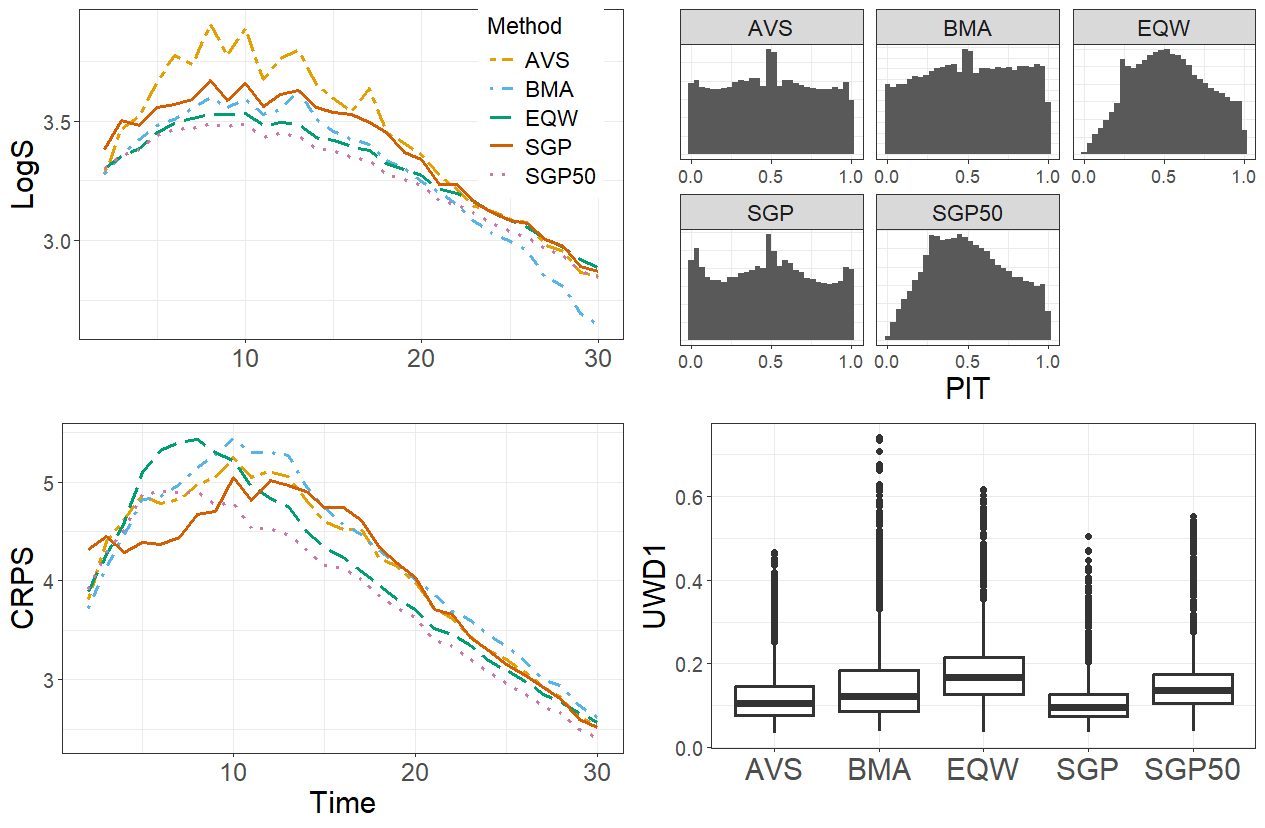
\includegraphics[width=.9\linewidth]{Images/sir_sim_res_col.png}
\caption{Plots showing results for one step ahead forecasts for SIR
data for the five
weighting methods SGP, SGP50, AVS, BMA, and EQW. Two plots show performance
according to proper scoring rules
(left). The mean LogS (top) and CRPS (bottom) over 3,000 replicates of one step
ahead predictions at 29 time points colored by weighting methods.
The other two plots show calibration according to the PIT (right). The PIT
histogram for all forecasts faceted by weighting method is shown (top), and
boxplots by weighting method of the UWD1 for all forecasts of one simulation
replicate is shown (bottom).}
\label{fig:sir_sim}
\end{figure}

The PIT histograms and boxplots in figure \ref{fig:sir_sim}
show that relative to the other methods, the SGP performs well in terms of 
forecast calibration. The SGP50 is less well calibrated and the histogram has a 
shape much closer to that of the EQW ensemble forecasts. In the supplementary 
materials an additional figure is included to compare the SGP and SGP50 
posterior weights for the component models in this study. The figure shows 
how the added regularization in the SGP50 brings posterior weights closer to
equality --in this case 1/4 since there are 4 component models-- but still 
allows for favoring some components over others.

The studies in this section show the SGP's ability to construct accurate 
forecasts for cases of both i.i.d. and dynamic data. The SGP largely 
outperformed AVS, 
BMA, and EQW ensembles both in terms of mean proper scoring rules and in PIT 
uniformity and calibration. 
The value of regularization to equal ensemble weights using a 
stronger prior distribution was also shown in the third study. 
In the next section, the SGP ensemble construction is applied 
to forecasts from the CDC FluSight, again with comparisons of 
performance against AVS, BMA, and EQW. 





\section{Analysis on 2023-24 CDC flu forecast competition} \label{sec:flu_analysis}

Every flu season, beginning in 2013 but with the exception of the 2020-21 flu 
season, the CDC has hosted a national flu forecasting competition, also known 
as FluSight. The competition begins in October and lasts around 30 weeks until
May of the following year. The competition generally involves 
a few dozen academic and 
industry research teams who each create separate probabilistic forecasts 
targeting certain flu events for future weeks. At the end of the season, 
forecast performance of all forecasts from each team are evaluated, and a 
winning team is announced 
\cite[]{mathis2024evaluation,biggerstaff2016results}. During the 2022-23 
and 2023-24 flu seasons, forecasts targeted 1, 2, 3, and 4-week ahead 
hospitalizations due to a laboratory confirmed flu infection for each of the 
50 US states, District of Columbia, Puerto Rico, and the nation as a whole. 
Every week during the competition, a team could submit a forecast for each 
target, and after the hospitalization count for the target was observed, the 
forecast was then scored and compared with all other forecasts. Besides 
reporting and scoring all forecasts individually, all submitted forecasts 
were combined into an ensemble forecast, which ensemble forecast 
was then published at 
\cite{cdc2024previous} as the official CDC forecast and scored along 
with the individual forecasts 
\cite[]{mathis2024evaluation,wadsworth2023mixture}.  

Teams were given complete freedom in how they developed their forecasts, 
and since the beginning of the competition there has been a large variety of 
methodologies used 
\cite[]{mathis2024evaluation,mathis2023flusight,mcandrew2021adaptively,
osthus2021multiscale,osthus2019dynamic,ulloa2019,morgan2018wisdom,
farrow2017human}. To make scoring and ensemble construction straightforward, 
each submitted forecast was required to follow a specified representation. 
During the 2022-23 and 2023-24 seasons, the requested forecast representation 
was a set of estimated quantiles for each of 23 probability values established 
by FluSight. For notation, we say each forecast team is given $K$ 
probabilities $0 \leq p_1, p_2, ..., p_K \leq 1$. Then, the $c^{th}$ 
competing team would submit quantiles --estimated however they please-- 
$q^{(c)}_{r,w+h,1}, ..., q^{(c)}_{r,w+h,K}$ where 
\[
    P(H_{r,w+h} < q^{(c)}_{r,w+h, k}) = p_k; \quad k \in (1, 2, ..., K)
\]
for $H_{r,w+h}$ hospitalizations in location or region $r$, for time horizon 
$h \in \{1,2,3,4\}$ weeks ahead, and where $H_{r,w}$ is the most recently 
observed hospitalization count at week $w$. 

The forecasts were scored by the weighted interval score (WIS), defined in 
(\ref{eq:wis}) \cite[]{bracher2021evaluating}. The WIS is a proper scoring 
rule made for scoring quantile or interval representation forecasts. In the 
definition, $P$ represents a probabilistic forecast with an interval 
representation including $I$ predictive intervals with different nominal 
levels. The values $v_0 = 1/2$ and $v_i = \alpha_i / 2$ are weights for 
each interval where $\alpha_i$ is the nominal level of the $i^{th}$ interval, 
$IS_{\alpha}$ is the interval score (IS) a proper scoring rule for a single 
interval as defined in (\ref{eq:is}), and $y^*$ is the true observation 
targeted by $P$.

\begin{equation}
\label{eq:wis}
        WIS_{0,I}(P, y^*) = \frac{1}{I + 1/2} \times 
        (v_0\times |y^* - median| + \sum_{k=1}^K \{v_i 
        \times IS_{\alpha_i}(P, y^*) \} )
\end{equation}

\begin{equation}
\label{eq:is}
        IS_{\alpha}(l,r;y^*) = (r-l) + 
        \frac{2}{\alpha}(l - y^*)\mathds{1}\{y^* < l\} + 
        \frac{2}{\alpha}(y^* - r) \mathds{1}\{y^* > r\}
\end{equation}
Like the CRPS, the WIS is a global scoring rule, allowing for evaluation over 
the whole range of the forecast. In fact, as the number of forecast intervals 
$I$ increases, the WIS becomes arbitrarily close to the CRPS 
\cite[]{bracher2021evaluating,gneiting2011comparing}. 

A drawback of the quantile representation and the WIS is that no information 
about the forecast distribution exists below the $1^{st}$ quantile or above 
the $K^{th}$ quantile. Another drawback is that even with a large number of 
quantiles, the information is less than would available from a PDF or CDF, 
and the quantile representation is not suited for scoring by the LogS or CRPS 
or ensembling building using a linear pool \cite[]{wadsworth2023mixture}.  
In order to apply the SGP from (\ref{eq:sgp}), which is based on the CRPS, 
the quantile 
Gaussian process quantile matching model from
\cite{wadsworth2025quantile} was fit to the quantiles to approximate a 
continuous
distribution from which the quantiles were estimated. This was done via 
Bayesian posterior Monte Carlo sampling from a normal mixture distribution. The 
result was 50,000 posterior predictive draws for forecasts of each location, 
week, and horizon. Monte Carlo approximations of the expected values in 
(\ref{eq:crps_ens_mse}) were calculated from the posterior predictive samples 
allowing for estimation of the CRPS for individual forecasts and ensemble 
forecasts. This allowed for using the SGP for selecting weights and 
constructing an ensemble forecast.

The analysis of ensemble forecasts of flu hospitalizations herein was limited 
to 1-week ahead forecasts. For each location, only the forecasts from teams 
who submitted forecasts for every week during FluSight were included 
so as to avoid dealing with missing forecasts. We expected that 
competing forecasts would vary in skill throughout the flu season and thus 
used the empirical risk function from (\ref{eq:er_dyn}) used in the dynamic 
setting. The FluSight candidate forecasts were dynamic, changing every week 
as the individual 
forecast teams updated their forecasts and the flu season progressed.
To complete the SGP, an uninformative Dirichlet prior with parameter 
$\mathbf{1}_C$ was assigned to $\boldsymbol{\omega}$. 
The SGP was fit via Hamiltonian 
Monte Carlo sampling using the \texttt{cmdstanr} \texttt{R} package 
\cite[]{stan2024manual,gabry2022stan}. To assess convergence of the fit, 
the SGP for US forecasts at the national level for the week of 
January 20, 2024 (week 15 of 29 of the flu season) was fit with 4 chains. 
Each chain consisted of 60,000 posterior draws, the first 10,000 draws being 
discarded as a burn-in. From this fit, among all posterior parameters, the 
largest $\hat{R}$ statistic \cite[]{vehtari2021rank} was 1.000055, giving 
no reason to be concerned about about MCMC convergence. The smallest 
effective sample size \cite[]{gelman2013bayesian} over all chains was 74,167. 
The SGPs for all other regions and weeks were fit using one chain of 60,000 
draws, the first 10,000 being discarded as a burn-in. The result was 50,000 
Monte Carlo vector draws for the weights $\{\omega^{(m)}\}_{m = 1}^M$.
For each $c$, the Monte Carlo mean of each weight 
$\bar{w}_{c,t} = M^{-1}w^{(m)}_{c,t}$ was calculated, and the mean weights 
were used in the ensemble forecast for hospitalizations at time $t+1$. 
Selecting the learning rate $\eta$ via cross validation did not appear to 
improve forecasts,
so $\eta$ was set to equal 1.
% selected by fitting the SGP for all forecasts up 
% to time $t-1$ and estimating model combination weights at all values of 
% $\eta$ on a pre-selected grid. The value of $\eta$ which produced combination 
% weights leading to the smallest CRPS of an ensemble model at time $t$ was 
% used in the SGP for time $t+1$.
Using this procedure, 1-week ahead ensemble forecasts were constructed for 
flu season weeks 2-29 for each location, noting that for the week 1 forecast 
ensemble, model weights were all selected to be equal. The CRPS was 
evaluated at the log forecast and log hospitalization. The mean CRPS for 
region $r$ across the season was calculated as
\[
    \overline{CRPS}(\bar{P}, \boldsymbol{H}_r) = 
    \frac{1}{W}\sum_{w = 1}^{W-1} CRPS(\bar{P}_w, H_{r,w + 1})
\]
for each region. A similar mean for each week where the average was over 
all regions was also calculated.


% \begin{figure}[hbt!]
%     \centering
%     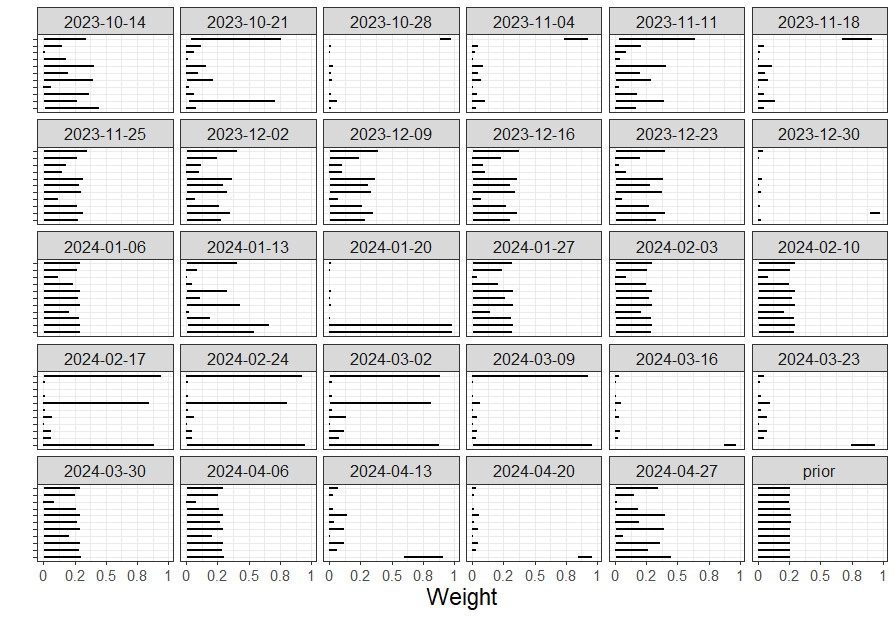
\includegraphics[scale=.5]{Images/us_post_int.png}
%     \caption{90\% credible intervals for forecast weights estimated via SGP 
%     for the 2023-24 CDC FluSite targetting flu hospitalizations at the 
%     national level of the United States. The intervals in the bottom right 
%     corner are those from the uninformative Dirichlet prior.}
%     \label{fig:us_wt_post_int}
% \end{figure}


The plots on the left of figure \ref{fig:flu_crps} shows 90\% SGP 
credible intervals for the 10 
included forecast models for flu hospitalizations for the state of 
Rhode Island --one of the regions where the SGP forecasts peprformed the best
relative to other methods--
for all weeks during the 2023-24 flu season. The plots show how the SGP model 
probabilities change through the season. At the beginning of the season, there
was little separation in probabilities for individual forecast weights, but
as the season progresses several component forecasts decrease in importance
while a few increase but with higher variability.
The plot on the right of figure \ref{fig:flu_crps} shows the mean CRPS 
scores for 
SGP, AVS, BMA and EQW divided by the mean CRPS score of the SGP
for all regions in one plot and over all weeks in the other. The value for 
SGP is thus always 1, and any value less than 1 for any other method 
is an instance of an ensemble 
method outperforming the SGP for one region.
In 31 
locations, the SGP ensemble forecasts has the best overall scores, and in
only 3 regions does the SGP perform the worst among the methods compared.


\begin{figure}[hbt!]
\centering
%\begin{subfigure}{}
  % \centering
  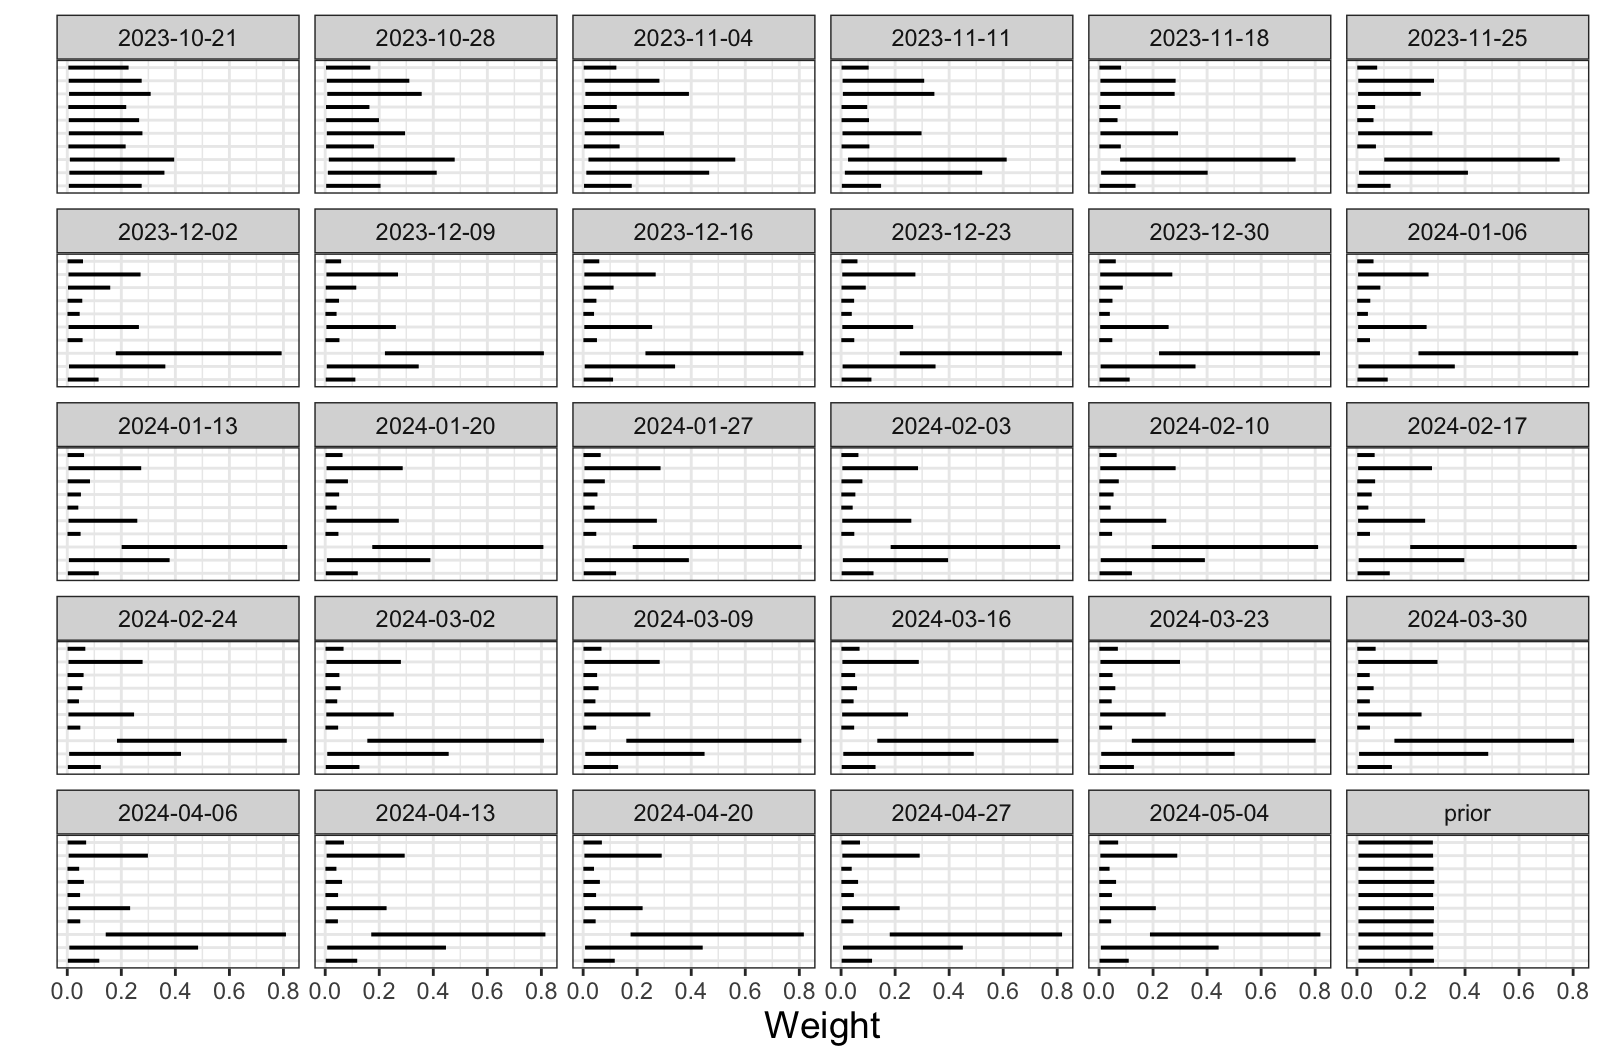
\includegraphics[width=.48\linewidth]{Images/ri_post_int.png}
  % \caption{A subfigure}
  % \label{fig:sub1}
%\end{subfigure}%
\hspace{0.01\textwidth}
%\begin{subfigure}{}
  \centering
  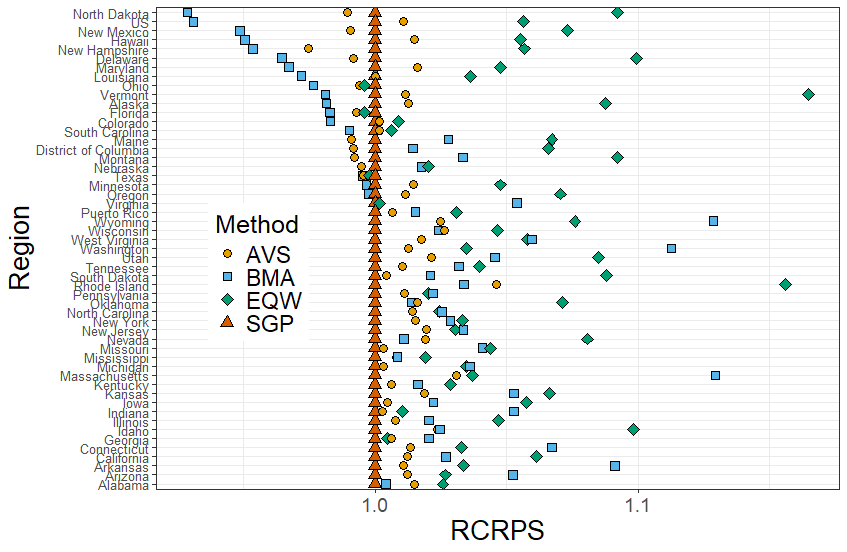
\includegraphics[width=.48\linewidth]{Images/real_data_rcrps.png}
  % \caption{A subfigure}
  % \label{fig:sub2}
%\end{subfigure}
\caption{90\% credible intervals for forecast weights estimated via SGP 
    for the 2023-24 CDC FluSite targetting flu hospitalizations at the
    national level of the United States (left). The intervals in the bottom 
    right
    corner are those from the uninformative Dirichlet prior.
Mean over regions CRPS for the four ensemble methods divided
by mean CRPS for the SGP
separated by shape and color (right).}
\label{fig:flu_crps}
\end{figure}


Table \ref{tab:forecast_rank} summarises the forecast performance for the 
four methods by showing in how many instances forecasts for each method were 
ranked 1, 2, 3, or 4 by mean CRPS over regions or weeks, a smaller 
ranking meaning better performance. 
By these rankings, SGP performed the best followed by BMA, AVS, and finally
EQW. 
In the supplementary material, a simlilar figure and table to 
% Figure \ref{fig:flu_wis} and table \ref{tab:forecast_rank_wis} are
% similar to those of 
figure \ref{fig:flu_crps} and table
\ref{tab:forecast_rank} show results for ensembles constucted via 
quantile averaging and forecasts scored by the WIS instead of the CRPS.


\begin{table}[h!]
\centering
\caption{Table showing the number of times ensemble forecasts for each method, 
SGP, AVS, BMA, and EQW, were ranked 1st, 2nd, 3rd, and 4th according to mean 
CRPS by region or week. There were 53
regions evaluated and 29 weeks, so each column under region should sum to 53
and each column under week to 29.}
 \begin{tabular}{cccccccccc}
 % {@{\extracolsep{\fill}}
 %    l
 %    *{8}{c}
 %    S[table-format=4.0]}
  Ranking
  & \multicolumn{4}{c}{By region CRPS}
  &
  & \multicolumn{4}{c}{By week CRPS} \\
  \cmidrule{2-5}  \cmidrule{7-10}
  & AVS & BMA & EQW & SGP & & AVS & BMA & EQW & SGP\\
  \midrule
  $1^{st}$ & 5 & 17 & 0  & \textbf{31} & & 5  & 8  & 2  & \textbf{14}\\
  $2^{nd}$ & 32 & 5 & 1  & 15 & & 17 & 4  & 0  & 8\\
  $3^{rd}$ & 16 & 17& 16 & 4  & & 7  & 10 & 8  & 3\\
  $4^{th}$ & 0 & 14 & 36 & 3  & & 0  & 7  & 19 & 3\\
  \bottomrule
 \end{tabular}
 \label{tab:forecast_rank}
\end{table}

% \begin{table}
% \caption{Table showing the number of times ensemble forecasts for each method, 
% SGP, AVS, BMA, and EQW, were ranked 1st, 2nd, 3rd, and 4th. There were 53 
% regions evaluated and 29 weeks, so each column under region should sum to 53 
% and each column under week to 29.}
% \begin{tabular*}{ccccccccc}
% {@{\extracolsep{\fill}}
%     l
%     *{8}{c}
%     S[table-format=4.0]}
%   Ranking
%   & \multicolumn{4}{c}{By region CRPS}
%   & \multicolumn{4}{c}{By week CRPS} \\
%   \cmidrule{2-5} \cmidrule{6-9}
%   & AVS & BMA & EQW & SGP & AVS & BMA & EQW & SGP\\
%   \midrule
%   $1^{st}$ & 0 & 0 & 0 & 53 & 1 & 0 & 0 & 28\\
%   $2^{nd}$ & 44 & 3 & 6 & 0 & 23 & 1 & 5 & 0\\
%   $3^{rd}$ & 7 & 3 & 43 & 0 & 5 & 0 & 24 & 0\\
%   $4^{th}$ & 2 & 47 & 4 & 0 & 0 & 28 & 0 & 1\\
%   \bottomrule
% \end{tabular*}
% \label{tab:forecast_rank}
% \end{table}

% \begin{figure}[hbt!]
% 
%     \centering
%     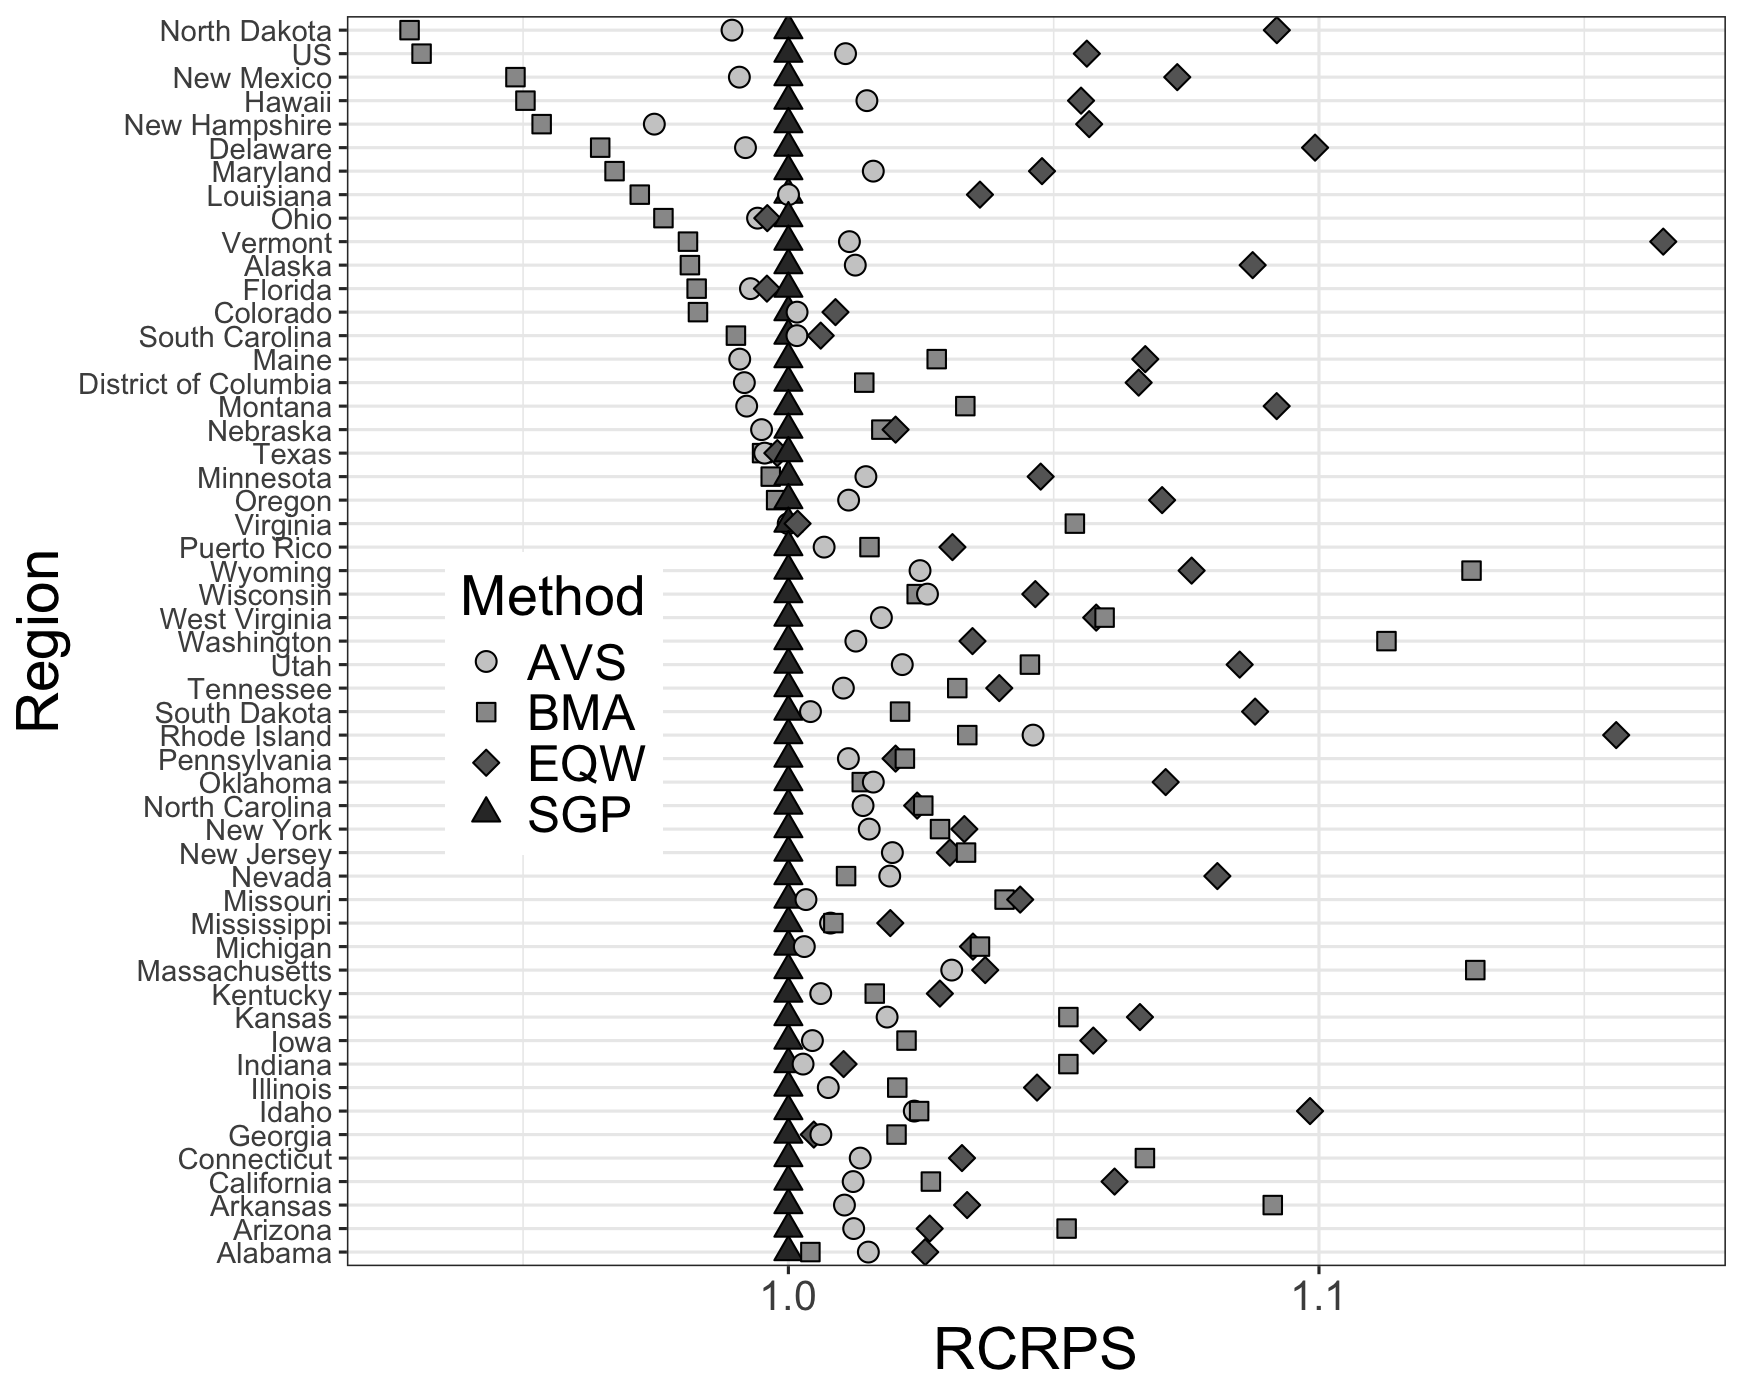
\includegraphics[scale=.45]{Images/flu_region_crps.png}
%     \caption{Average CRPS for linear pooled forecast across all weeks of the 2023-24 influenza season for all 53 regions. Stacking weighting methods are separated by shape/colour.}
%     \label{fig:opt_dens}
% \end{figure}


This analysis demonstrates the effectiveness of selecting weights for a 
linear pooled ensemble forecast by optimizing the dynamic risk function in 
(\ref{eq:er_dyn}) via the SGP. Given that the forecasts 
used were posterior predictive samples from a model fit on quantile 
forecasts, it was key to be able to make a Monte Carlo approximation of the 
CRPS from (\ref{eq:crps_ens_mse}). Of the methods compared, the SGP is 
arguably the most complicated, but in forecast performance it more often than 
not outperformed the other methods. 


\section{Discussion} \label{sec:4conc}

In this manuscript, we introduced a new method for optimizing model weights 
in a linear pooled forecast ensemble. The method, which is based on 
optimization of the CRPS using a Gibbs posterior distribution, provides 
uncertainty quantification for optimal linear pool weights and allows for a 
prior distribution to inform and influence weight selection. Included with 
the development of the SGP is a theorem for the asymptotic consistency of 
the Gibbs posterior. The SGP was used in three simulation studies and a data 
analysis on the 2023-24 FluSight forecasts to evaluate performance for model 
weighting, and it was compared with two posterior model averaging methods 
and an equally weighted linear pool ensemble. Performance of the methods was 
determined by forecast performance in terms of minimizing the CRPS and LogS, 
and in the second and third simulation studies 
by analyzing the uniformity of the PIT. 
In the simulation studies and the flu forecast analysis, the SGP showed 
superior forecast 
performance when compared to the AVS, BMA, and EQW. In the third simulation 
study, a more informative prior distribution showed the value of regularization
of ensemble weights to be equal.

The promising results show that the SGP is a valuable contribution to the 
field of probabilistic forecast combination. The content of the SGP explored 
in this paper was primarily directed at forecasting a future event, but in 
a scenario where ensemble component model uncertainty is of more concern, 
further exploration 
of the Gibbs posterior should be carried out. This may include further 
exploration into the selection or design of objective prior distributions 
\cite[]{giummole2019objective}. 
Other aspects of the SGP to be explored could be its use on scoring rules 
other than the CRPS or in nonlinear model combination methods. While the 
CRPS is a popular and useful measure of probabilistic forecast performance 
and one which we show is often simple to estimate in the continuous mixture 
distribution case, other scoring rules exist and different rules may be 
preferable for use in different applications. The WIS, for example, remains 
the preferred scoring method of the quantile forecasts for FluSight. An 
adaption of the SGP where the empirical risk is based on the WIS instead of 
the CRPS may be better suited for FluSight and other forecast hubs. Likewise, 
optimizing the linear pool forecast model in (\ref{eq:linp_forc}) may not 
be the ideal method for ensemble building. In fact the linear pool, while 
relatively simple to construct, has its drawbacks such as the difficulty of 
producing a completely uniform PIT \cite[]{gneiting2013combining}. 
Applications of the SGP in the context of the so called generalized linear 
pool would be another direction of further development.

A limitation of this work is the asymptotic consistency theory of the SGP. 
Theorem \ref{thm:sgp_cons} is limited to the case where the data is i.i.d. 
and where the models of the linear pool are fixed. An issue with posterior 
consistency in the dynamic setting is the tendency for the skill of 
probabilistic forecast models to vary in time making a single risk minimizer 
unlikely to exist without strict assumptions. Another limitation, present in 
the flu forecast application, is that forecasts are often missing. In the 
analysis in section \ref{sec:flu_analysis}, only models with 100\% submission 
over the course of the flu season for a given region were included in 
the ensemble forecasts. Over the 
season, many forecast teams failed to submit forecasts during some weeks, 
and even if their forecasts were highly skilled these could not be included 
in the SGP 
as it is developed here. Modifying the SGP to account for missing forecasts 
so that they may factor into an ensemble when included, or by considering 
any of the above recommendations could improve the overall performance 
and/or lead to additional developments.




\section{Acknowledgments}
This work is partially supported by the National Science Foundation under 
Grant No. 2152117. Any opinions, findings, and conclusions or recommendations 
expressed in this material are those of the author(s) and do not necessarily 
reflect the views of the National Science Foundation.

% Include this in the Bayesian Analysis submission
% \begin{supplement}
% Supplement to ``Bayesian
% Stacking via Proper Scoring Rule
% Optimization using a Gibbs Posterior``\\
% A. Additional plots from first simulation study\\
% % \end{supplement}
% B. Additional plots from second simulation study\\
% C. Weighted interval score results from 2023 FluSight
%  forecast analysis
% \end{supplement}

\bibliographystyle{ba}
\bibliography{master_bib}

%%%%
% Reference section comes before the appendix

%\bibliographystyle{acm} % use for numbered citations along with options given in preamble. Look at the main thesis.tex file
% \bibliographystyle{apa}
% \bibliography{master_bib}


% \jarad{Check all references for accuracy, capitalization.}
% %\section{Bibliography}
% \bibliographystyle{apa}
% % \vspace{-20pt}
% \begingroup
%     \setlength{\bibsep}{13.2pt}
%     \linespread{1}\selectfont
%     \bibliography{master_bib}
% \endgroup
% \clearpage
% \pagebreak

%%%%%
%% Appendix
% This section may or may not be included
% Chapter 2 shows a double appendix example. Please use A or B as in Appendix A if there are multiple appendix. Use "Appendix A:" before writing the title
% Chapter 3 shows a single appendix example. Use "Appendix:" before writing the title 
\section{Appendix: Proofs of proposition \ref{prop:crps_ens_mse} and theorem 
\ref{thm:sgp_cons}}

\subsection{Proof of proposition \ref{prop:crps_ens_mse}} \label{app:crps_ens_pf}

\begin{proof}
The random variables $X$ and $X'$ in (\ref{eq:crps_mse}) are independent 
copies of the same random variable with mixture distribution PDF 
\[
\bar{p}(x) = \sum_{c = 1}^C w_c p_c(x)
\]
where each $p_c(x)$ is a PDF of a continuous random variable. The random 
variables $X_c$ and $X'_c$ are independent copies of a random variable with 
PDF $p_c(x)$. Then the second expectation in (\ref{eq:crps_mse}) is  
    \begin{flalign*}
        E|X - X'| &= \int_{\mathcal{X}} \int_{\mathcal{X}} |x - x'| p(x)p(x') 
        dxdx' \\
        &= \int_{\mathcal{X}} \int_{\mathcal{X}} |x - x'| 
        \sum_{i = 1}^C w_c p_c(x) \sum_{d = 1}^C w_d p_d(x') dx dx' \\
        &= \sum_{c = 1}^C \sum_{d = 1}^C w_cw_d \int_{\mathcal{X}} 
        \int_{\mathcal{X}} |x-x'|p_c(x)p_d(x') dx dx' \\
        &= \sum_{c = 1}^C \sum_{d = 1}^C w_cw_d E|X_c-X'_d|
    \end{flalign*}
Similary for the first expectation
\[
    E|X - y| = \sum_{c = 1}^C w_c E|X_c - y|
\]
and the result in (\ref{eq:crps_ens_mse}) follows.
\end{proof}



\subsection{Proof of theorem \ref{thm:sgp_cons}} \label{app:sgp_cons_pf}
\begin{proof}
\cite{martin2022direct} identify three sufficient conditions needed to prove 
Gibbs posterior consistency. The first is that the prior distribution give 
sufficient mass to the risk minimizer $\omega^*$. This is met with the selected 
Dirichlet prior. The other two conditions are a uniform law of large numbers 
and a separation or identifiability condition. Respectively these two 
conditions are (\ref{eq:cons_ull}) and (\ref{eq:cons_sep}).
\begin{equation}
    \underset{\omega \in \Omega}{\text{sup}} |G_n(\omega) - G(\omega)| 
    \rightarrow 0 \text{ in } \mathcal{L}-\text{probability}
    \label{eq:cons_ull}
\end{equation}

\begin{equation}
    \underset{\omega:d(\omega, \omega^*) > \delta}{\text{inf}} \{G(\omega) - 
    G(\omega^*)\} > 0 \text{ for any } \delta > 0
    \label{eq:cons_sep}
\end{equation}

\noindent We first show (\ref{eq:cons_ull}). By lemma 2.4 in 
\cite{newey1994large}, if 
\begin{enumerate}[i)]%[\hspace{.5cm}i)]
    \item the data are iid
    \item $\Omega$ is compact
    \item $CRPS(\bar{P}_{\omega}, y)$ is continuous at each $\omega \in 
    \Omega$ with probability 1
    \item there is a function $m(y)$ such that $|CRPS(\bar{P}_{\omega}, y)| 
    \leq m(y)$ and $E[m(Y)] < \infty$
\end{enumerate}
then $G(\omega)$ is continuous and (\ref{eq:cons_ull}) follows. Conditions i) 
and ii) are met by assumption and iii) is met by the continuity of the CRPS.
To show iv) we let
\begin{align*}
    \text{CRPS}(\bar{P}_{\omega}, y) &= E|X - y| - \frac{1}{2}E|X - X'| \\
    &\leq E|X - y| \\
    &\leq E\left[|X| + |y|\right] \\
    &=E|X| + |y| := m(y)
\end{align*}
Then by the assumption that $E|Y| < \infty$, $E[m(Y)] < \infty$ meeting 
condition iv) and showing (\ref{eq:cons_ull}).

Now to show (\ref{eq:cons_sep}). Consider the open set $B_{\delta'} = 
\{\omega : d(\omega, \omega^*) < \delta'\}$ and the closed set 
$\overline{B}_{\delta} = \{\omega : d(\omega, \omega^*) \leq \delta\}$ 
where $0 < \delta' < \delta$. Since $B_{\delta'}$ is open, the set 
$\Omega \setminus B_{\delta'} \subset \Omega$ is a closed subset of a 
compact set and is thus compact. Because  $G(\cdot)$ is continuous, the 
set $G(\Omega \setminus B_{\delta'})$ is also compact and thus contains 
its infimum. Now $\Omega \setminus \overline{B}_{\delta} \subset \Omega 
\setminus B_{\delta'}$, so $G(\Omega \setminus \overline{B}_{\delta'}) 
\subset G(\Omega \setminus B_{\delta'})$. Thus 
\[
     G(\omega^*) < \underset{\Omega \setminus B_{\delta'}}{\text{inf}} 
     G(\omega) \leq \underset{\Omega \setminus 
     \overline{B}_{\delta}}{\text{inf}} G(\omega)
\]
and (\ref{eq:cons_sep}) holds.
\end{proof}



% Now we show (\ref{eq:cons_sep}). To do this, we first show that (\ref{eq:crps_ens_mse}) is a convex function in $\Omega$. For $0 < \nu < 1$, $\omega, \omega^* \in \Omega$ 

% \begin{align*}
%     CRPS(\bar{P}_{\nu \omega + (1 - \nu) \omega^*}, y) &= \\
%     &\quad \sum_{c = 1}^C (\nu w_c + (1 - \nu)w_c^*)E|X_c - y|\\ 
%     &- \frac{1}{2} \sum_{c = 1}^C \sum_{c' = 1}^C (\nu w_c + (1 - \nu)w^*_{c})(\nu w_{c'} + (1 - \nu)w^*_{c'})E|X_c - X_{c'}| \\
%     & = \nu \sum_{c = 1}^C w_c E|X_c - y| + (1 - \nu)\sum_{c = 1}^C w^*_c E|X_c - y| \\
%     &-\frac{1}{2}\sum_c \sum_{c'} \left[\nu^2 w_c w_{c'} + (1 - \nu)^2w_c^* w_{c'}^*\right]E|X_c - X_{c'}|\\
%     &-\frac{1}{2} \sum_c \sum_{c'}E|X_c - X_{c'}|\left[\nu (1 - \nu)w_c w_{c'}^* + \nu (1 - \nu)w_c^* w_{c'}\right] \\
%     &\leq \nu \sum_{c = 1}^C w_c E|X_c - y| + (1 - \nu)\sum_{c = 1}^C w^*_c E|X_c - y| \\
%     &-\frac{1}{2}\sum_c \sum_{c'} \left[\nu^2 w_c w_{c'} + (1 - \nu)^2w_c^* w_{c'}^*\right]E|X_c - X_{c'}|
% \end{align*}

% \begin{align*}
% \nu CRPS(\bar{P}_{\omega}, y) &+ (1 - \nu) CRPS(\bar{P}_{\omega^*}, y) =\\
% & \nu \left[ \sum_c w_c E|X_c - y| - \frac{1}{2}\sum_c \sum_{c'} w_c w_{c'} E|X_c - X_{c'}|\right] \\
% &+ (1-\nu) \left[ \sum_c w^*_c E|X_c - y| - \frac{1}{2}\sum_c \sum_{c'} w^*_c w^*_{c'} E|X_c - X_{c'}|\right]
% \end{align*}


% \end{proof}
% Show that 
% \[
%     \sup_{\theta \in \Theta} | R_n(\theta) - R(\theta) | \overset{p}{\rightarrow} 0
% \]

% where $\l_{\theta}(y) = CRPS(F,y)$

% \begin{align*}
%     \text{CRPS}(F, y) &= \int_{-\infty}^{\infty} \left(F(x) - \mathds{1} (y \leq x)\right)^2 dx \\
%     &= \int_{-\infty}^y(F(x) - 1)^2 dx + \int_y^{\infty} F(x)^2 dx \\
%     &= \int_{-\infty}^y P(X > x)^2 dx + \int_y^{\infty}P(X \leq x)^2 dx
% \end{align*} 

% Nevermind the above do the following instead

% \begin{align*}
%     \text{CRPS}(F, y) &= \int_{-\infty}^{\infty} \left(F(x) - \mathds{1} (y \leq x)\right)^2 dx \\
%     &= E|X - y| - \frac{1}{2}E|X - X'| \\
%     &\leq E|X - y| \\
%     &\leq E\left[|X| + |y|\right] \\
%     &=E|X| + |y|
% \end{align*}

% If $E|X| < \infty$, $E_Y|y| < \infty$ then 3 is met in Lemma 2.4 Newey and Mcfadden 1994 (Handbook of econometrics) and 

% \[
%   \sup_{\theta \in \Theta} \left|\frac{1}{n}\sum_{i = 1}^n CRPS(F, y_i) - E[CRPS(F, Y)]\right| \overset{p}{\rightarrow} 0
% \]

% Now I need to show that under the CRPS that if there is a unique $w^*$ at which for $E[CRPS(F_{w^*}, Y)] = R(w^*) < R(w) = E[CRPS(F_{w}, Y)]$ for all $w$, then 
% \[
%     \inf_{w:d(w, w^*) > \delta} \{R(w) - R(w^*)\} > 0
% \]
% for any $\delta > 0$ where $d(x, y)$ is the Euclidean norm. For all $w:d(w, w^*) > \delta$, one may construct
% \[
%     w' = w^*  + \frac{\delta}{d(w,w^*)}(w - w^*) = \frac{\delta}{d(w,w^*)}w + \left(1-\frac{\delta}{d(w,w^*)}\right)w^*
% \]
% Note that $0 < \delta/d(w, w^*) < 1$. $R(w)$ is convex, so
% \[
%     R(w') \leq \frac{\delta}{d(w,w^*)}R(w) + \left(1-\frac{\delta}{d(w,w^*)}\right)R(w^*) \leq R(w)
% \]
% Now $w' \in \Omega' = \{w : d(w, w*) = \delta \} \subseteq \Omega \setminus B(w, \delta)$ 
% where
% $B(w,\delta) = \{w \in \Omega : d(w, w*) > \delta \}$ so for all $w \in B(w, \delta)$ there exists a $w' \in \Omega'$ such that $R(w') <= R(w)$, hence $\inf_{w \in \Omega'} R(w) <= \inf_{w \in B(w, \delta)} R(w)$, and since $\Omega'$ is compact it achieves its infimum and $\inf_{w \in \Omega'} R(w) > R(w^*)$ and 
